\documentclass[letterpaper,twocolumn]{article}

\usepackage[top=1in,bottom=1in,left=0.75in,right=0.75in]{geometry}
\usepackage{graphicx}
\usepackage{multirow}
\usepackage{newtxtext}
\usepackage{newtxmath}
\usepackage{pifont} % For checkmarks in tab:nat-matching.
\usepackage[hyphens]{url}
\usepackage[table]{xcolor}

\usepackage[textsize=footnotesize]{todonotes}\setlength{\marginparwidth}{1.5cm}

% Better look for citations that include a section reference like \cite[\S 3]{foobar}.
\usepackage{cite}
\renewcommand{\citemid}{~}

% Load hyperref after other packages.
\usepackage[pdfa,hidelinks,pdfcreator={},pdfproducer={}]{hyperref}
\urlstyle{same}
\def\sectionautorefname{Section}
\def\subsectionautorefname{Section}

% Disable metadata for reproducible PDF.
% https://tex.stackexchange.com/a/313605
\usepackage{ifpdf}
\ifpdf
\pdfinfoomitdate=1
\pdftrailerid{}
\pdfsuppressptexinfo=-1
\fi

\hyphenation{Web-RTC}
\hyphenation{Web-Exten-sion}
\hyphenation{Java-Script}
\hyphenation{uProxy}

% Highlight the first usage or definition of a technical term.
% Like the firstterm element in DocBook: https://tdg.docbook.org/tdg/5.2/firstterm.html.
\newcommand{\firstterm}[1]{\textit{#1}}

\begin{document}

\date{}

\title{Snowflake, a censorship circumvention system \\using temporary WebRTC proxies}

\author{}

\maketitle

\begin{abstract}
Snowflake is a system for circumventing Internet censorship.
It~derives its blocking resistance from
the use of numerous, ultra-light, temporary proxies (``snowflakes''),
which accept traffic from censored clients using peer-to-peer WebRTC protocols
and forward it to a centralized bridge,
which does the real work of directing traffic to its destination.
The temporary proxies are lightweight enough to be implemented in JavaScript,
in a web page or browser extension,
making them vastly cheaper to set up than
a traditional proxy or VPN server.
The proxies are not assumed to have stable network addresses
or be online all the time,
and even the blocking of currently in-use proxy
is not fatal to a circumvention session,
as the system permits clients to switch proxies on the fly.

% Need anything about broker, centralization here?

Snowflake has been deployed with success
in Tor Browser and Orbot for several years.
It has been significant for circumvention
during high-profile network disruptions,
including in Russia in~2021 and Iran in~2022.
In this paper, we explain the composition of Snowflake's many parts,
give a history of deployment and attempts to block~it,
and reflect on implications for circumvention generally.
\end{abstract}

% General references:
%   https://keroserene.net/snowflake/technical/#history
%   https://www.bamsoftware.com/papers/thesis/#chap:snowflake

\section{Introduction}
\label{sec:intro}

Censorship circumvention systems
may be characterized on multiple axes.
There are those that seek to avoid blocking
by imitating some common, high-value protocol;
and those that randomize their protocols
in order not to look like any other protocol in particular.
Some concentrate their traffic into one, or a few,
well-known proxies, somehow entangled with other traffic
such that a censor cannot easily block them;
and others that spread their traffic out over
hundreds or thousands of proxies,
none of which is individually difficult to block,
but which are difficult for a censor to discover and block in their entirety.
What all circumvention systems have in common
is that they strive to increase the \emph{cost}
to the censor of blocking them---whether that be
in the form of research and development,
human resources, and hardware,
or in the inevitable overblocking that results
when a censor tries to block circumvention traffic
that is difficult to distinguish from other traffic
the censor values highly.
On the spectrum of mimicry to randomization,
Snowflake falls more on the mimicry side;
on the scale of concentrated to diffuse,
it is diffuse.
If~Snowflake has a single distinguishing characteristic,
it is that it pushes this idea of distributed, disposable
proxies to an extreme,
by making proxies extremely cheap to run,
in web browsers, using WebRTC to communicate.

WebRTC is a suite of interacting protocols
intended to enable real-time communication applications
in web browsers~\cite{rfc8825}.
Video and voice chat are familiar and typical examples
of WebRTC applications.
Snowflake exchanges WebRTC data formats
in the course of establishing a connections,
and uses WebRTC protocols for NAT traversal
and for data transfer between the client and a temporary proxy.
Critically for Snowflake, WebRTC protocols
are exposed by JavaScript APIs in web browsers,
meaning it is possible to implement a WebRTC-based proxy
in an ordinary web page or browser extension.
WebRTC is also usable outside a browser,
which is how we implement the Snowflake client program
and alternative, command line--based proxies.

As is typical in circumvention research,
we assume a threat model where
censored \firstterm{clients} reside in a censor-controlled network.
The \firstterm{censor} has the power to inspect and interfere with
traffic that crosses the border of its network;
in practice, this power takes the form of things like
inspection of IP addresses and destination server hostnames,
dynamic protocol detection,
IP address blocking, and injection of false DNS responses
or TCP RST packets.
The client wants to exchange some information with a
destination outside the censor's network---often
with the assistance of third-party \firstterm{proxies}---and
the censor is motivated to block either the contents
of the communication, or the destination itself.
The censor is aware of the possibility of circumvention,
and therefore seeks not only to block direct access,
but also indirect access by way of a proxy or proxy protocol.
We consider circumvention to be accomplished when a client
can reliably reach any proxy,
because the proxy then provides access to any desired destination.
(In Snowflake, we separate the roles of temporary \firstterm{proxies}
and a stable long-term \firstterm{bridge}, but the idea is the same.)
Mitigating in the client's favor
is the fact that the censor is presumed to derive some benefit
from permitting some forms of network access:
the censor cannot trivially ``win''
simply by blocking all connections,
but must be selective in what to block and allow
in order to optimize some objective of its own.
The art of censorship circumvention is
forcing the censor into a difficult dilemma
of overblocking or underblocking,
by making circumvention traffic difficult to distinguish
from traffic that the censor finds valuable.

Snowflake has its origin in two earlier projects:
flash proxy and uProxy.
% https://lists.torproject.org/pipermail/tor-dev/2016-January/010310.html "Snowflake is a webrtc pluggable transport inspired by flashproxy."
% https://keroserene.net/snowflake/technical/#1-introduction "It is inspired by and builds upon the previous work of Flashproxy. Snowflake is much like a hybrid of previous Pluggable Transports..."
Flash proxy~\cite{Fifield2012a}, like Snowflake, used a model
of untrusted, temporary JavaScript proxies running in web browsers;
however the link between client and proxy was WebSocket
rather than WebRTC.
(WebSocket still finds use in Snowflake,
but only on the proxy--bridge link,
not the client--proxy link.)
Flash proxy was deployed in Tor Browser
% 2013: https://blog.torproject.org/combined-flash-proxy-pyobfsproxy-browser-bundles
% 2016: "Remove Flashproxy from Tor Browser" https://bugs.torproject.org/17428#note_2203210
from 2013 to~2016,
but it never saw much use,
probably because the reliance on WebSocket,
which are TCP-based and do not have built-in NAT traversal like WebRTC does,
and required uses to perform a
% https://gitlab.torproject.org/legacy/trac/-/wikis/doc/PluggableTransports/FlashProxy/Howto
cumbersome port forwarding procedure.
WebRTC was at the time an emerging technology, and while
% "Investigate WebRTC for flash proxy NAT punching" https://bugs.torproject.org/5578
% flashproxy.pdf §5.2: "New technologies like WebRTC [24] may fill this need in the future, if they become sufficiently popular that flash proxies' use of them does not stand out as unusual."
it was considered as a future transport protocol for flash proxy,
it was decided to begin Snowflake as a new, separate project,
rather than build atop flash proxy.
% https://serene.cx/snowflake/#note-flashproxy "...one could say that uProxy and flashproxy are the ancestors of snowflake."
uProxy~\cite{uproxy}, in one of its early incarnations,
% "in one of its earlier incarnations": uProxy pivoted from friend proxies to cloud servers in 2016:
%  https://web.archive.org/web/20161211194847/https://blog.uproxy.org/2016/02/get-access-24x7-through-your-own-uproxy.html
pioneered the use of WebRTC proxies.
uProxy's proxies were browser-based,
but the trust and deployment model was rather different
from flash proxy's and Snowflake's.
There was no centralized proxy discovery;
instead each censored client would arrange, out of band,
% uProxy v1.2.5 Design Doc: https://docs.google.com/document/d/1t_30vX7RcrEGuWwcg0Jub-HiNI0Ko3kBOyqXgrQN3Kw
% "uProxy depends on leveraging existing trust relationships to to find and use a proxy."
for a personal acquaintance, outside the censor's network,
to run a proxy in their web browser.
The social trust relationship was necessary to prevent misuse,
because the browser proxies fetched destination content directly,
without any further intermediary like the bridge in Snowflake.
A~uProxy proxy was expected to be
persistent and always online;
clients did not changes proxies on the fly.
% https://github.com/uProxy/uproxy-obfuscators
uProxy supported protocol obfuscation:
though the communication protocol was fundamentally WebRTC,
the contents of packets could be transformed so as not to resemble WebRTC.
This was possible because uProxy ran as a privileged browser extension
with access to socket operations.
Since Snowflake uses ordinary unprivileged browser APIs,
its WebRTC is restricted to looking like WebRTC;
on the other hand, because of that,
it is even easier to deploy a Snowflake proxy.
Like flash proxy, uProxy was active in the years
% 2013: Serene's 30C3 lightning talk on uProxy https://events.ccc.de/congress/2013/wiki/Static:Lightning_Talks#Day_3
2013--2016\todo{Check 2016 end date for uProxy}.

The closest existing system to Snowflake is MassBrowser~\cite{Nasr2020a}.
% https://github.com/net4people/bbs/issues/32
It incorporates many circumvention techniques, one of which is
proxying though volunteer proxies, called buddies.
The architecture is similar to Snowflake's:
there is a centralized component responsible for coordinating
connections between clients and proxies called the operator,
like Snowflake's broker;
MassBrowser buddies correspond to our snowflake proxies.
The trust model is intermediate between those of Snowflake and uProxy:
buddies may provide proxy service to strangers and not only their social acquaintances,
but buddies specify categories of content they are willing to directly proxy,
in order to mitigate misuse.
Buddies preferentially operate as one-hop proxies,
but also support proxying into a Tor bridge, as in Snowflake;
this option, however, is treated as a last resort rather than a default mode,
in keeping with MassBrowser's guiding principle of
of prioritizing blocking resistance and performance
over anonymity and privacy.
An~innovation in MassBrowser not present in Snowflake is client-to-client proxying:
clients may act as buddies for other clients,
with the reasoning that what is censored for one client may not be censored for another.
The buddy software is standalone application software,
which means that it, like uProxy, can use protocol obfuscation
% V-D: "We also implement traffic obfuscation to protect MassBrowser's traffic
% against traffic analysis attacks. Particularly, we have built a custom
% implementation of the obfsproxy Tor pluggable transport tailored to work with
% our MassBrowser implementation."
% VI-A: "MassBrowser uses a custom protocol over TCP/UDP for the communications
% between Clients and Buddies."
on the client--buddy link.
Like Snowflake, MassBrowser has been deployed to real users
and tested in practice against censors.
Protozoa~\cite{Barradas2020a}
% https://github.com/net4people/bbs/issues/55
is superficially similar
to Snowflake in its use of WebRTC,
but the two systems are essentially different.
More like uProxy, Protozoa has a one-to-one proxy model:
client and proxy discover one another and arrange a connection out of band,
and the proxy persists as long as the client is using it.
If Snowflake's specialty is diversity of proxy addresses,
Protozoa's is traffic analysis:
using an authentic WebRTC audio or video stream as a carrier,
it replaces the content of encrypted, encoded media frames
with covert ciphertexts of the same length,
such that the replacement is undetectable to an observer.
One technical subtlety is that where Snowflake uses
WebRTC data channels,
Protozoa uses WebRTC media streams,
which may be an advantage;
we will return to this point in \autoref{sec:fingerprinting}.
\todo{Check if \href{https://censorbib.nymity.ch/\#Figueira2022a}{Stegozoa}
and \href{https://censorbib.nymity.ch/\#Barradas2020b}{CRON} are relevant,
and discuss if so.}

% Very early versions of Lantern (circa 2014) used social network–based trusted proxies:
%   https://web.archive.org/web/20140326223853/http://techpresident.com/news/wegov/24455/why-remarkably-similar-circumvention-tools-uproxy-and-lantern-are-not-overkill
%   https://lists.torproject.org/pipermail/tor-dev/2014-March/006356.html "HOWTO use Lantern as a pluggable transport"
%   https://web.archive.org/web/20130831160152/https://www.youtube.com/watch?v=aiPkCugE-RY
%   https://web.archive.org/web/2oe_/http://wayback-fakeurl.archive.org/yt/aiPkCugE-RY
% But it wasn't WebRTC, so was less like Snowflake than uProxy was.
% I'll draw the line here, since even Tor bridges are "volunteer-operated" in a sense.

There is a tendency in writing about
circumvention research to disproportionately emphasize
the deficiencies of other systems
and the advantages of one's own.
It may give an impression to the reader
that the state of censorship circumvention
is more dire than it really is.
Such is not our aim.
While challenges remain,
today's circumvention systems are largely successful
and work in the situations people need them to.
For many people, circumvention is just another part of their
day-to-day use of the Internet.
With Snowflake, we are exploring a different point in the design space,
one with a different set of tradeoffs of advantages and disadvantages,
but not categorically superior in every dimension.
Here we present not only the design of Snowflake
and the principles that explain why it should be hard to block,
but also the experience of deployment on a large scale.
A~great deal of the interest in this kind of research
is in the complications that emerge when idea meets practice.

\todo{Origin of the name Snowflake?}
\todo{Deployed since\ldots\allowbreak \(X\)~TB per month\ldots}

\section{How it works}
\label{sec:mechanics}

\begin{figure*}[t]
\framebox[\textwidth]{\vbox to 2in{\vfil\centering TODO\vfil}}
\caption{
Architecture of Snowflake.
}
\label{fig:architecture}
\end{figure*}

A~Snowflake proxy connection proceeds in three phases.
First, there is the rendezvous, where a client
signals its need for circumvention service
and is matched with a temporary proxy.
Then, there is connection establishment,
where the client and its temporary proxy connect to one another
with WebRTC, using information exchanged during rendezvous.
Finally, there is data transfer,
where the proxy ferries data back and forth
between the client and a remote service
(e.g., a Tor bridge).
\autoref{fig:architecture}
illustrates the process.

The client's circumvention session
does not begin and end with any particular temporary proxy.
Rather, the client strings together
a series of proxies, switching to a new one
whenever an old one goes offline.
This proxy handoff is hidden from the upper-layer protocols
(i.e., the web browser) that use the circumvention tunnel:
to them the Snowflake session appears as one long unbroken connection.

There is an ambient population of temporary Snowflake proxies.
For the most part, these proxies are the web browsers of people who have
installed the Snowflake proxy WebExtension,
or a functionally equivalent headless command-line version.
The proxies periodically poll a centralized server, the broker,
to inquire whether there are any clients that need service.
The broker is responsible for matching and
keeping track of associations between clients and proxies.

A~client begins a Snowflake session by
sending a rendezvous message to the broker.
The rendezvous message must be sent over a blocking-resistant channel,
which may however be slow or expensive; see \autoref{sec:rendezvous} for some examples.
When a client rendezvous message arrives,
the broker chooses one of the immediately available proxies,
subject to NAT compatibility and other matching criteria,\todo{Are there other matching criteria?}
forwards the client's rendezvous message to that proxy,
and conveys the client's downstream answer to the rendezvous back to the client.
The client and proxy then initiate a WebRTC connection
with each other; the broker is no longer involved.
Further details on rendezvous will be presented in \autoref{sec:rendezvous}.

The temporary proxy connects both to its assigned client
and to a centralized bridge,
and begins to copy bytes between the client and the bridge
in both directions.
Details about how the connections are established are in \autoref{sec:ice}.
This continues until the client ends its session by disconnecting,
or the proxy goes offline
(which happens, for example, when the web browser where a proxy is running is closed).
When a proxy goes offline,
it does not spell the end of the client's session:
the client and the bridge share end-to-end session state
that persists beyond the lifetime of any single proxy.
The client sends another rendezvous message to the broker,
is assigned another proxy,
and picks up where it left off.
More information about the data transfer phase is in \autoref{sec:data-transfer}.

Never does the client communicate with the broker or bridge directly.
Both the broker and the bridge may be blocked,
from the perspective of the client.
The client only communicates with the broker over an indirect rendezvous channel
that is assumed to be difficult and expensive for a censor to block.
The client only communicates with the bridge via a temporary proxy.
No single temporary proxy is critical to the operation of the system.
A~proxy may be blocked---even while it is in active use by a client---and
clients can adapt by using a different proxy.

\subsection{Rendezvous}
\label{sec:rendezvous}

In the first phase of establishing a Snowflake circumvention session,
the client exchanges a small amount of information with a server
outside the censor's zone of control,
in a process called rendezvous.
It is not possible for a Snowflake client
to establish a peer-to-peer WebRTC connection
with a temporary proxy straight away.
(For one thing, neither the client nor the proxy
know a network identifier for each other at the outset.)
The client and proxy bootstrap a connection between them
by way of a separate blocking-resistant channel
(i.e., something other than WebRTC)
and an intermediary known as the broker.

Rendezvous is not unique to Snowflake;
it is a fairly common component of circumvention designs.
Precedents include the
DEFIANCE Rendezvous Protocol~\cite[\S 3]{Lincoln2012a}
the facilitator interaction in flash proxy~\cite[\S 3]{Fifield2012a},
and the registration proxy in Conjure~\cite[\S 4.1]{Frolov2019b}.
Even commercial VPNs built on commodity protocols
often require contacting some kind of API server
before initiating a connection, which can also be considered rendezvous.
A~key property of rendezvous-using systems
is that they do not rely on any preshared secret information.
The client user needs only to acquire the necessary software;
whatever additional information is required to establish a circumvention session
is exchanged dynamically, at runtime.
A~corollary of the no-secret-information property
is that an adversary---the censor---has
no special disadvantage in attacking the system:
they may download the client software
and then act in every way as a normal user.
This is in contrast to other systems in which,
after acquiring the necessary circumvention software,
a~client must also get ahold of some secret,
such as a password or proxy address,
through an out-of-band channel
presumed to be unavailable to the censor---and
blocking resistance hinges on that secret information
remaining unknown to the censor.
In rendezvous-based systems like Snowflake,
if the censor does not block a proxy server,
it is not out of ignorance,
but because the censor is constrained in some other way,
for example by computational limitations
or fear of collateral blocking.

If rendezvous has the advantage of not requiring secrecy,
its disadvantage is that it presents one more thing to worry about.
Not only the main data transfer channel
but also the rendezvous channel must resist blocking:
the system as a whole is only as secure as the weaker of the two.
The saving grace here is that the security and performance requirements
of rendezvous are different, and generally more lenient.
Rendezvous can afford to be relatively more heavyweight,
slow, expensive, or inefficient for the sake of blocking resistance,
because it accounts for only a small fraction of the overall communication
and occurs only intermittently.
The enlarged design space of rendezvous encompasses
forms of data hiding that would be impractical
for bulk data transfer.
Another helpful consideration is that rendezvous protocols
are separable from the rest of the system.
The assumption of using WebRTC is embedded fairly deeply in Snowflake;
but the rendezvous part is modular,
not coupled to WebRTC or even any single other protocol.

Snowflake rendezvous requires a bidirectional exchange:
the client sends one message to the broker, then receives
one message in reply.
(This is a step backward from flash proxy,
which required only one outgoing message for its rendezvous,
but the communication model of WebRTC makes a reply message unavoidable.)
It is therefore a good fit for request--response protocols,
like those based on HTTP.
We currently support two rendezvous methods in Snowflake:

\begin{description}
\item[Domain fronting]
In this method, the client does one HTTPS exchange
with the broker; however routing through an intermediary such as a CDN,
and disguising the externally visible domain name\todo{Audit ``domain name'' vs.\ ``hostname''.}
(the TLS Server Name Indication, or SNI) so that the exchange
appears to be destined to a different site~\cite{Fifield2015a}.
The well-known drawback of domain fronting
is the high financial cost of CDN bandwidth,
but because we use it only for rendezvous and not bulk data transfer,
the cost is vastly lower than it would be in a system like~meek.
\item[AMP cache]
% https://gitlab.torproject.org/tpo/anti-censorship/pluggable-transports/snowflake/-/merge_requests/50
AMP is a framework for web pages written in a restricted dialect of HTML.
Part of this framework is a free-to-use
cache server~\cite{amp-cache}.
Because the cache fetches upstream pages on demand,
it works as a specialized sort of HTTP proxy.
By encoding rendezvous messages as AMP-conformant HTML,
we can use the cache as a proxy for rendezvous,
one that is not easily blocked without blocking the cache server as a whole.
This rendezvous method still requires domain fronting,
because the AMP cache protocol would otherwise expose the
upstream server's domain name in the TLS SNI,
but it increases the number of usable intermediary nodes.
\end{description}

The rendezvous component is, however, modular,
and any system that can be persuaded to indirectly convey a request
of about 1500 bytes, and a response of about the same size,
can work as a plug-in rendezvous method.
% https://bugs.torproject.org/tpo/anti-censorship/pluggable-transports/snowflake/25594
For example, encrypted DNS
% https://bugs.torproject.org/tpo/anti-censorship/pluggable-transports/snowflake/25874
% \cite[\S 3.4]{Fifield2020a}
(DNS over TLS or DNS over HTTPS):
the client encodes its registration message as a series of DNS queries;
the broker acts as an authoritative resolver;
and a third-party recursive resolver acts as an indirect intermediary,
while DNS encryption hides the broker's domain name in queries
from external observers.
% Flash proxy email rendezvous would not work for Snowflake, because unidirectional.
% https://gitweb.torproject.org/flashproxy.git/tree/flashproxy-reg-email
% https://gitweb.torproject.org/flashproxy.git/tree/facilitator/fp-registrar-email

A~Snowflake rendezvous message is a serialized bundle of data.
Its essential element
is the information necessary to establish a WebRTC connection,
namely a Session Description Protocol (SDP) \firstterm{offer}~\cite{rfc8839}.
The offer contains information needed for a network connection,
such as the client's external IP addresses;
as well as cryptographic information to secure a later key exchange between the peers.
% Specifically, a certificate fingerprint: https://www.rfc-editor.org/rfc/rfc8122.html#section-5
The rendezvous message also contains the client's
self-measured NAT type, which the broker will use to try to match it
with a compatible proxy.
The client serializes all these pieces of data and sends them to the broker.
The broker chooses an available proxy
and forwards the client's offer to it.
The proxy composes an SDP \firstterm{answer},
containing its own external addresses and cryptographic information,
and sends it back to the broker,
which then forwards it to the client.
Having exchanged an offer and answer,
the client and proxy are now able to establish a direct WebRTC connection,
without the broker in the middle.
The gathering of external IP addresses
forms part of the ICE protocol
and uses third-party STUN servers,
\todo{Should say more about STUN and gathering of ICE candidates here.}
which are described in more detail in \autoref{sec:ice}.

In WebRTC terms, the offer/answer exchange is called
``signaling,'' and the broker here acts as a signaling server.
While signaling is a necessary component
of any WebRTC-based system,
there is no specified way of doing it.
Every application must invent its own signaling system
according to its requirements
(which for us include covertness and blocking resistance).
Because of the lack of uniformity in accomplishing signaling,
the way a WebRTC application does (or does not do) signaling
may be a distinguishing feature; see \autoref{sec:fingerprinting}
for more considerations along these lines.

\begin{figure}
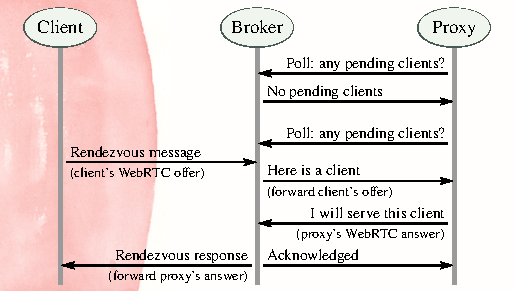
\includegraphics{figures/rendezvous/rendezvous}
\caption{
The long-polling communication model of Snowflake rendezvous.
The assigned proxy connects twice in between the time
the client sends its message and receives the response;
to the client it looks like one roundtrip.
Here, the client's rendezvous method is abstracted;
in reality the censor never contacts the broker directly,
but only via an intermediary.
The shaded background shows the censor's zone of control.
}
\label{fig:rendezvous}
\todo[inline]{Replace provisional graphic.}
\end{figure}

We use a ``long polling'' model for the client's side of broker interaction.
See \autoref{fig:rendezvous}.
There are proxies polling the broker constantly.
Each poll is an HTTPS request to a designated URL path.
(We assume there is no need for covertness
in the proxies' interaction with the broker,
because this side is outside the censor's observation and control.)
On receiving a poll request,
the broker does not send an HTTPS response immediately,
but waits for a few seconds to see if a client will become available.
If not, the broker sends a response saying ``no clients''
and the proxy sleeps for a while before trying again.
If a client rendezvous does arrive,
the broker extracts the SDP offer and forwards it to the proxy
in the HTTPS response.
The proxy computes its SDP answer,
then sends it back to the broker in a new HTTPS request
(with an attached identifier to permit the broker to match it
with the earlier polling request.)
Meanwhile, the client has been waiting for a response
to its rendezvous message.
The broker encapsulates the proxy's SDP answer
and sends it to the client over the rendezvous channel,
and simultaneously sends an acknowledgement to the proxy.
Now that the client and proxy have each other's
SDP information, they are ready to actually connect to one another.

\subsection{Peer-to-peer connection establishment}
\label{sec:ice}

After rendezvous,
a censored client in need of service
and a temporary snowflake proxy
will have exchanged
(among other information)
their IP addresses,
using the broker as an intermediary.
After this point, the broker is no longer involved
(as~far as that specific client--proxy pairing goes).
The next step is for the client and proxy
to establish a direct connection---which
is not a trivial operation,
even in the absence of censorship,
because of possible interference by
network address translation (NAT)
and ingress filters at either endpoint.
(Recall that many proxies run in web browsers
in ordinary residential ISPs,
without the connectivity of a typical Internet server.)
WebRTC is designed for exactly this use case
and has built-in facilities for traversing NAT.
Specifically, WebRTC uses
ICE (Interactive Connectivity Establishment)~\cite{rfc8445},
a procedure for testing candidate pairs of peer network addresses
until finding one that works.
ICE~makes use of
STUN (Session Traversal Utilities for NAT)~\cite{rfc8489}
and third-party STUN servers that provide services such as,
for example, allowing a network host to
discover its own external IP addresses.
In~Snowflake, candidate IP addresses are gathered
during rendezvous, with the assistance of STUN servers,
and sent as part of rendezvous messages.
ICE~may also use
TURN (Traversal Using Relays around NAT)~\cite{rfc8656},
effectively a UDP proxy.

There is no guarantee that two arbitrary peers will be able to make
a connection using the facilities of STUN alone.
Some mapping and
filtering setups are simply incompatible with one other.
Most uses of ICE would fall back to TURN in this case,
inserting a relay server between the peers to resolve any difficulties.
TURN is problematic for Snowflake,
because TURN relays' IP addresses are
generally fixed and easily discoverable by a censor.
% "Configure TURN servers for the proxy and/or client" https://bugs.torproject.org/tpo/anti-censorship/pluggable-transports/snowflake/25596
But there is a factor working in our favor:
a client does not need to be matched to a \emph{specific} proxy;
any compatible proxy will~do.
In Snowflake, client and proxies self-assess their NAT configuration.
Then the broker takes care to pair clients
with proxies that they are most likely to be able to connect to directly.

% "Investigate Snowflake proxy failures" https://gitlab.torproject.org/tpo/anti-censorship/pluggable-transports/snowflake/-/issues/33666#note_2595319
% "Okay here's a summary of what I've found: ..."

Snowflake clients and proxies have one of a few possible
network configurations that can be categorized by two factors:
the mapping behavior of its NAT,
and the filtering behavior of its firewall.
The implementation details of how NATs map internal IP address and port combinations
to external ports varies significantly, but for our purposes it suffices
to condense these variations, together with common firewall filtering behaviors,
into the following well-known NAT variations:

\begin{description}
\item[Full cone]
All connections from the same internal IP address
and port are mapped to the same external IP address and port. Any remote
host may send a packet to an internal host by sending a packet to the
mapped external IP--port pair.
\item[Restricted cone]
Like full-cone NAT,
except that incoming packets
are allowed only if
there has been a recent outgoing packet
to the same remote IP address.
\item[Port-restricted cone]
Like restricted-cone NAT,
except that incoming packets are allowed only if
there has been a recent outgoing packet
to the same remote IP--port pair.
\item[Symmetric]
The external IP--port pair depends on both
the internal IP--port pair and the external IP--port pair.
Incoming packets are allowed only if
there has been a recent outgoing
packet to the remote address.
\end{description}

\begin{table}
\definecolor{Ycolor}{Gray}{14}
\definecolor{ncolor}{Gray}{13}
\newcommand{\Y}{\cellcolor{Ycolor}\ding{51}}
\newcommand{\n}{\cellcolor{ncolor}--}
\newcommand{\rotlabel}[1]{\rotatebox{45}{#1}}
% \vphantom is to make the labels take up vertical space;
% \rlap is so they don't expand the horizontal size of table columns.
\newcommand{\rot}[1]{\vphantom{\rotlabel{#1}}\rotlabel{\rlap{#1}}}
\centering
\begin{tabular}{@{}rccccc@{\hspace{1.5ex}}l@{~}l@{}}
& % empty
\rot{No NAT} &
\rot{Full cone} &
\rot{Restricted cone} &
\rot{Port-restricted cone} &
\rot{Symmetric} &
&
\\
No NAT               & \Y & \Y & \Y & \Y & \Y & \multirow{3}{*}{$\left.\rule[-12pt]{0pt}{24pt}\right\}$} & \multirow{3}{*}{\small ``unrestricted''} \\
Full cone            & \Y & \Y & \Y & \Y & \Y & \\
Restricted cone      & \Y & \Y & \Y & \Y & \Y & \\
Port-restricted cone & \Y & \Y & \Y & \Y & \n & \multirow{2}{*}{$\left.\rule[-7pt]{0pt}{14pt}\right\}$}  & \multirow{2}{*}{\small ``restricted''} \\
Symmetric            & \Y & \Y & \Y & \n & \n & \\
\end{tabular}
\caption{
Pairwise compatibility of NAT types for connection establishment with STUN.
The incompatible cases are when one peer's NAT is symmetric
and the other's is symmetric or port-restricted.
}
\label{tab:nat-matching}
\todo[inline]{Update this figure with one that shows how the ``restricted'' and ``unrestricted'' label is allotted differently for clients and proxies.}
\todo[inline]{Check style guide to see if caption should be before or after a table.}
\end{table}

Table~\ref{tab:nat-matching}
shows the pairwise compatibility of NAT variations.
As the incompatible cases always involve a symmetric NAT,
we further simplify matching by categorizing the NAT type of peers as either
``unrestricted'' (i.e., works with most other types of NATs) and ``restricted''
(i.e., works only with the more permissive NATs). For load-balancing reasons,
we categorize port-restricted NATs differently for proxies and clients.
Proxies are considered ``restricted'' if they have a port-restricted cone NAT
or a symmetric NAT, and ``unrestricted'' otherwise. Clients are considered
``restricted'' only if they have a symmetric NAT. This wasn't always the case; the
use of different categorizations was motivated by the scarcity of ``unrestricted''
proxies. Because port-restricted NATs work with other port-restricted NATs and are
prevalent in the proxy pool, we decided to save the ``unrestricted'' proxies for
symmetric NAT clients. Our measurements show that clients with port-restricted NATs
can still connect to around 80\% of ``restricted'' proxies and will establish a working
connection in a reasonable amount of time.\todo{measure that 80\% number again}

We determine the NAT and firewall behavior of snowflake peers
differently for clients and proxies, due to
limitations in browsers and potential censorship vectors that
only matter for client connections.
For clients, we use the NAT discovery feature in STUN~\cite{rfc5780}.
% "Use STUN to determine NAT behaviour of peers" https://bugs.torproject.org/tpo/anti-censorship/pluggable-transports/snowflake/34129
% "Add utility to help user discover their NAT type" https://github.com/pion/stun/issues/8
Not all STUN servers support NAT behavior discovery,
but we ensure that those whose addresses we ship with the Snowflake client~do.
If NAT discovery fails, the client will classify their NAT type as ``unknown''.
The client reports its NAT type to the broker
in its rendezvous message.
The broker conservatively assumes that clients
with an ``unknown'' NAT type have a symmetric NAT.
Most clients work well with the majority of Snowflake proxies, as
shown in \autoref{fig:client-nat}.
However, approximately one quarter of client polls
self report having a restricted NAT type.\todo{Double check this number and update if needed.}

\begin{figure}[t]
\includegraphics[width=\columnwidth]{figures/clients-by-nat}
\caption{Snowflake client poll counts by NAT type.}
\label{fig:client-nat}
\todo[inline]{Replace provisional figure.}
\todo[inline]{Commit source data (e.g.\ CSV) to repository.}
\bigskip
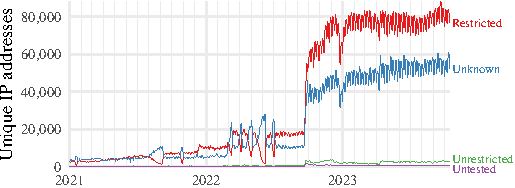
\includegraphics{figures/proxies/proxy-nat-type}
\caption{
Unique proxy IP addresses per day,
by NAT type.
}
\label{fig:proxy-nat}
\todo[inline]{Explain temporary inversions of restricted and unknown (\href{https://bugs.torproject.org/tpo/anti-censorship/pluggable-transports/snowflake/40071}{\#40071}, \href{https://bugs.torproject.org/tpo/anti-censorship/pluggable-transports/snowflake/40147}{\#40147}).}
\end{figure}

We use a different technique to determine the NAT type of Snowflake proxies,
because the NAT behavior discovery feature
is not exposed in the WebRTC API available to web browsers.
% "Have a remote probe service to test snowflake proxy NAT compatability" https://bugs.torproject.org/tpo/anti-censorship/pluggable-transports/snowflake/40013
We adapt a technique from MassBrowser~\cite[\S \mbox{V-A}]{Nasr2020a},
and have proxies attempt to establish a connection with a peer under our control,
which is behind a simulated symmetric NAT.
If the connection is successful,
the proxy's NAT type is ``unrestricted''
and it is eligible to be matched with any client;
if not, it is ``restricted''
and may only be matched to known ``unrestricted'' clients.
Clients and proxies
retest their NAT type periodically, to account for changes in their local networking
environment.

We have a number of
mechanisms in place to avoid too much reliance on single points of failure.
When a proxy cannot determine its NAT type,
it is conservatively assumed to be ``restricted'' and the broker distributes it
along with proxies with known restricted NATs.
If a proxy was previously able to determine its NAT type,
a~failure of a periodic retest will not cause it to revert to ``unknown'' status.
A~proxy that self-tests as unrestricted,
but which nevertheless fails multiple client connections in a row,
will reclassify itself as restricted
until its next successful NAT check.

The majority of browser-based Snowflake proxies
fall into the ``restricted'' category.
\autoref{fig:proxy-nat} shows the distribution of proxies by NAT type.
\todo{Consider moving \autoref{fig:client-nat} and \autoref{fig:proxy-nat} to \autoref{sec:experience} so as not to slow the pace here.}
Despite this, we have managed to maintain a sufficient number of unrestricted proxies,
thanks in large part to the standalone, command-line
version of the Snowflake proxy,
which tends to be run on rented VPSes in less restricted networks.
\todo{Perhaps dwell on the duality here:
standalone proxies knowingly sacrifice some address diversity
for better NAT compatibility in a common case.}

At the same time as the snowflake proxy makes a connection to its assigned client,
% "At the same time": https://gitlab.torproject.org/tpo/anti-censorship/pluggable-transports/snowflake/40228
it also connects to the bridge.
In~contrast to the client--proxy link,
the proxy--bridge link
uses the WebSocket protocol~\cite{rfc6455}, not WebRTC.
WebSocket offers a TCP-like, point-to-point, client--server connection
layered atop HTTPS.
As we assume the danger from a censor is past
once a client reaches a snowflake proxy,
the choice of protocol for the next hop to the bridge is somewhat arbitrary.
It just needs to be a protocol that is supported in browsers
and has reasonable performance.
WebRTC would fit the bill for this link too,
but WebSocket is somewhat less complex and easier to program.

At the end of this phase,
a temporary snowflake proxy has made two connections,
one to its client and one to the bridge.
It~then proceeds to proxy a data stream between them
in both directions,
until the client terminates the session,
or the proxy itself stop operating
(when the web browser it is running in closes, for example).

\subsection{Data transfer}
\label{sec:data-transfer}

No complicated processing takes place at the proxy.
The main value if a snowflake proxy is its IP address---it
gives the client somewhere to connect to that the censor does not know about yet.
Having provided that, the proxy assumes a role
of pure data transfer until it, or one of the endpoints, goes away.
Snowflake proxies are simple conduits that transfer
a bidirectional data stream between endpoints,
without interpreting~it.
In particular, the proxy may not interfere with any
end-to-end secure information exchanged between client and bridge,
which in our deployment using Tor,
includes not only the contents of the client's streams
but also their eventual destination.
It~may be considered an instance of the
``untrusted messenger'' model described by
Feamster et~al.~\cite[\S 3]{Feamster2003a}:
what they call a ``messenger'' is our snowflake proxy;
their ``portal'' is our bridge.

The full stack of protocol layers is shown below.
We will describe each one and its purpose
in the paragraphs that follow.

\begin{verbatim}
UDP  \ WebRTC       \
DTLS | data channel | ephemeral, per proxy
SCTP /              /
KCP  \ Turbo        \
smux / Tunnel       | persistent, per session
Tor protocol        /
client streams
\end{verbatim}
\todo[inline]{Redraw ASCII art as a proper figure.}

Communication between the client and the snowflake proxy
takes place over
a WebRTC data channel~\cite{rfc8831}, which
provides a TCP-like
reliable stream interface over a UDP-based carrier.
Reliability comes from an embedded layer of
Stream Control Transmission Protocol (SCTP), which
does reordering and retransmission of dropped packets---similar
to what an OS kernel does for a TCP connection,
but in userspace.
SCTP packets are then encapsulated in Datagram TLS (DTLS)~\cite{rfc9147}
for confidentiality and integrity between the WebRTC peers.
The peers mutually authenticate one another
at the DTLS layer using certificate fingerprints
that were exchanged during rendezvous~\cite[\S 5.1]{rfc8842}.
DTLS records are placed in UDP datagrams for transport.
The UDP--DTLS--SCTP combination comes as a packaged unit
that cannot be decomposed using the interfaces available to web browsers.

Data channels are a convenient abstraction for Snowflake,
because transmission of reliable,
connection-oriented streams data is closely matched
to the use case of a circumvention proxy.
But data channels are not the only available option:
WebRTC also provides media stream,
for unreliable transmission of real-time audio and video.
Data channels and media streams have distinguishable wire representations
that give rise to fingerprinting concerns we take up in \autoref{sec:fingerprinting}.

If snowflake proxies were as reliable as traditional proxies,
what we have described so far would already suffice:
send client traffic through the WebRTC data channel,
and have the proxy relay it to the bridge.
But Snowflake's temporary proxies might
disappear at any moment,
and the design must account for that.
If the client is in the middle of a long download,
for example, the failure of a proxy should not interrupt it:
the client and the bridge need a shared notion of session state
that is independent of any single temporary proxy connection,
so that the download can be resumed where it left off,
once connectivity is restored on a new proxy.
A~lack of session persistence across temporary proxies
was an unsolved problem in flash proxy~\cite[\S 5.2]{Fifield2012a}.

To make this possible, we employ the
Turbo Tunnel design pattern~\cite{Fifield2020a};
that is, we interpose an additional, userspace,
session/reliability layer between the raw transport layer
and client application streams.
This additional layer gives the proxy and the bridge
shared end-to-end state that persists throughout
the sequence of temporary proxies that are the carriers of a Snowflake session.
For the embedded session/reliability layer
we use a combination of
KCP~\cite{kcp} and
smux~\cite{smux}:
KCP provides reliability and reordering,
and smux detects the end of idle sessions and terminates them.
There is nothing essential about KCP/smux;
any other transport protocol that provides the necessary features
and can be implemented in userspace would~do,
such as QUIC, TCP, or (another layer of) SCTP.
(In~fact, we prototyped successfully with QUIC, before settling on KCP/smux.)
The Turbo Tunnel layer does not depend on any browser features,
because its packets are encapsulated into the data channel;
from the proxy's point of view, it's just a sequence of bytes.
A~switch from one temporary proxy to another
is invisible to the upper application layers,
except for a brief delay in packet delivery.
The failure of a proxy
is not fatal to a Snowflake session,
just as a dropped packet does not mean the end of a TCP connection.

Snowflake's Turbo Tunnel layer
is partially redundant with the data channel SCTP layer
on the WebRTC link between client and proxy,
which similarly builds a reliable stream interface
on an unreliable substrate.
\todo{Clarify/\allowbreak refine this in light of the fact that
\href{https://lists.torproject.org/pipermail/anti-censorship-team/2023-March/000286.html}{data channels can be unreliable and unordered}.
% "turn off reliable mode for WebRTC DataChannel" https://gitlab.torproject.org/tpo/anti-censorship/pluggable-transports/snowflake/-/merge_requests/109
% "Snowflake is currently using network resource in a so suboptimal way..." https://bugs.torproject.org/tpo/anti-censorship/pluggable-transports/snowflake/40251#note_2891751
}
The duplication is, in any case, unavoidable:
the data channel's SCTP layer is walled off by abstractions
in the WebRTC APIs available to browsers.
But more significantly, Snowflake requires an
\emph{end-to-end} notion of a session,
between the client and the bridge,
whereas the WebRTC data channel is only a
\emph{hop-by-hop} session
whose lifetime is tied to a single temporary proxy.

The combination of data channels and an inner Turbo Tunnel layer
provide a long-lasting ``virtual'' connection between the client and the bridge
that is composed of a sequence of ``real'' connections through temporary proxies.
Conceptually, here Snowflake's circumvention task is finished:
the client only needs to somehow tell the bridge, through the tunnel,
what resources to fetch, and the bridge fetches them and returns them through the tunnel.
Practically, we need to specify some concrete proxy protocol to fill this role.
This is another place where anything reasonable will serve,
with the caveat that it should be an encrypted protocol
(secure between client and bridge) to prevent proxies
from inspecting or interfering with the client's requests.
(The client--proxy link is encrypted with DTLS
and the proxy--bridge link with HTTPS,
but in the middle of these the proxy is in a position to see
the client's traffic, unless separately end-to-end encrypted.)
Our deployment is built on Tor,
and the bridge in our deployment is a Tor entry relay.
The Tor client provides a local SOCKS interface,
which fills the role of an encrypted proxy protocol,
and users of course get Tor's anonymity and privacy benefits
in addition to the blocking resistance supplied by Snowflake.
(In our deployment, not even the bridge is fully trusted---it
does not get to see the contents of clients' connection,
nor their eventual destinations.)
But there is nothing about Tor that Snowflake depends on essentially;
the tasks of providing a blocking-resistant to the bridge
and then telling the bridge what to do are easily separable.
We~discuss alternatives to Tor
and other extensions of Snowflake in \autoref{sec:future}.
Integration with Tor brings its own challenges,
which we will get into in \autoref{sec:challenges}\todo{Check this cross reference when \autoref{sec:experience} is fleshed out.}.

\section{Protocol fingerprinting}
\label{sec:fingerprinting}

% https://gitlab.torproject.org/tpo/anti-censorship/pluggable-transports/snowflake/-/wikis/Fingerprinting

Snowflake leans heavily into the ``address blocking'' side of blocking resistance,
but the ``content blocking'' part matters too.
As always, the goal is to make circumvention traffic
difficult to distinguish from traffic the censor cares not to block.
Snowflake is, by nature, tied to WebRTC,
and therefore can only be effective against a censor
that cannot afford to block WebRTC protocols wholesale.
But even within that scope,
there are many possible variations in \emph{how}
WebRTC is implemented and used,
which, if not considered carefully, might permit a censor
to selectively block only Snowflake,
while leaving other uses of WebRTC undisturbed.
In~this discussion, it is worth remembering
what Tschantz et~al.\ have observed\cite[\mbox{VI-A}]{Tschantz2016a}:
that censors prefer to exploit
simple, precise, deterministic distinguishers
that appear in the early phase of a circumvention session whenever possible,
and use long-term, probabilistic, or computationally expensive tests
only as a last resort.
It is hardly worth worrying about protocol fingerprints
in a circumvention system while easier distinguishers exist;
conversely, small, corrigible fingerprinting flaws may be excused
as long as the foundation is solid.

As~WebRTC is designed for the web,
most implementation of WebRTC are embedded in web browsers,
and are not trivially usable outside that context.
Snowflake originally used a WebRTC library extracted from Chromium,
but that eventually proved unworkable from a practical standpoint---more
details are in \autoref{sec:deployment}.
Since 2019, Snowflake has used Pion~\cite{pion-webrtc},
% "Evaluate pion WebRTC" https://bugs.torproject.org/tpo/anti-censorship/pluggable-transports/snowflake/28942
an independent implementation of WebRTC
implemented as a generic library,
not tied to any browser.
This is both good and bad.
The good is greater agility and less development friction,
and a working relationship with upstream developers
that enables us to get fingerprinting-related changes made.
The bad is that the WebRTC fingerprint of Pion
does not automatically match that of the primarily browser-originated
WebRTC that Snowflake aims to blend in with.

Unfortunately for the circumvention developer,
the rich set of interacting protocols that comprise WebRTC
afford a large attack surface for fingerprinting.
Not only that, WebRTC leaves the details of
the signaling path---where peers exchange information
needed to set up a connection,
corresponding to Snowflake rendezvous---unspecified~\cite[\S 3]{rfc8825},
leaving applications to invent their own mechanisms.
% "The choice of protocols for client-server and inter-server signaling, and the definition of the translation between them, are outside the scope of the WebRTC protocol suite described in this document."
% https://www.rfc-editor.org/rfc/rfc8829.html#section-3.1: "JSEP does not specify a particular signaling model or state machine, other than the generic need to exchange session descriptions in the fashion described by [RFC3264] (offer/answer)..."

The following is a list of potential fingerprinting concerns
that bear on Snowflake, together with brief descriptions
of the degree to which we have tried to address them.
The list may not be exhaustive.

\begin{description}
\item[Selection of STUN servers]
It~is not unusual for a WebRTC application to use STUN;
but which servers it uses is externally observable
and is the choice of the application (often hardcoded).
Running a dedicated STUN server just for Snowflake is a nonstarter---if~there
are no users of the server other than circumvention users,
a~censor will experience no harm in simply blocking its IP address.
In~Snowflake, we use a pool of public STUN servers,
used for many purposes other than circumvention,
and filtered for those that support the NAT behavior discovery feature
described in \autoref{sec:ice}.
The client chooses a random subset of the servers in the pool
each time it makes a connection.
This is because not every STUN server is accessible
under every censor.
% I went to check stun.l.google.com for blocking in China,
% but OONI Probe does not measure that server as of v3.17.1:
% https://github.com/ooni/probe/issues/2417#issuecomment-1468478811

\item[Format and content of STUN messages]
STUN messages consist of a fixed header
followed by a variable-length list of ordered
attributes~\cite[\S 5]{rfc8489}.
STUN is most often deployed using plaintext UDP as a transport,
which leaves its messages open to inspection
and potentially fingerprintable.
What attributes appear,
and their relative order,
is a property of the the implementation
and the way the application uses STUN.
Among the attributes are some used
for the NAT behavior discovery feature~\cite[\S 7]{rfc5780}
of \autoref{sec:ice}.

\todo{Have we done anything for STUN message fingerprinting?}
% "Investigate if STUN over TCP/TLS is beneficial to us" https://bugs.torproject.org/tpo/anti-censorship/pluggable-transports/snowflake/40240

\item[Rendezvous]
The rendezvous methods of
\autoref{sec:rendezvous},
being modular,
generally all need their own security argument
as to why they should be difficult to block.
Besides that, each must be implemented in a way
that does not expose accidental distinguishers.
For example, the domain fronting and AMP cache rendezvous methods
use HTTPS, which is TLS, which means they are susceptible to TLS fingerprinting~\cite[\S 5.1]{Fifield2015a}.
In Snowflake, we use the uTLS package~\cite[\S VII]{Frolov2019a}
(commonly used by circumvention programs)
to get a TLS fingerprint that is randomized or that imitates common browsers.
See \autoref{sec:block-ir} for an account of when
domain fronting rendezvous was briefly blocking in Iran,
because we were slow in activating uTLS.

Though each rendezvous method must be difficult to block in itself,
a~censor may combine a low-confidence suspicion of having observed a rendezvous exchange
with features from other phases of the Snowflake data exchange
to strengthen its guess and possibly effect a blocking decision.

\item[DTLS]
The outermost protocol
of a WebRTC data connection, exposed to the censor,
is Datagram TLS (DTLS) over UDP.
DTLS is an adaptation of TLS~\cite[\S 1]{rfc9147},
and inherits the fingerprinting concerns of the latter~\cite{Frolov2019a}.
TLS/DTLS fingerprinting may involve, for example,
inspecting the ClientHello message to see what
ciphersuites and extensions are used,
and their ordering---it may be that a particular fingerprint
is specific to a particular implementation of a circumvention system
and may therefore be blocked at low cost to the censor.

Due to practical implementation considerations,
the defenses to DTLS fingerprinting in Snowflake are not very robust,
and are reactive rather than proactive.
In~the world of TLS one may use the uTLS package~\cite[\S VII]{Frolov2019a},
or~(at a not inconsiderable cost of complexity)
tunnel through a locally installed web browser
to borrow its TLS fingerprint~\cite[\S 5.1]{Fifield2015a}.
But there is as yet no equivalent of uTLS for DTLS,
and using a browser's DTLS implementation proved unworkable
even for implementation, let alone convenient deployment to users.
The present way of altering DTLS fingerprints in Snowflake
is by submitting pull requests to the Pion project
whenever a fingerprint feature actually used for blocking is identified.
\autoref{sec:block-ru} documents how this has happened twice,
in response to blocking in Russia.

% For reference, fingerprinting changes upstreamed to Pion:
% * IP addresses as SNI values
%   https://bugs.torproject.org/tpo/anti-censorship/pluggable-transports/snowflake/40014#note_2764715
%   https://github.com/pion/dtls/issues/406
%   https://github.com/pion/dtls/pull/407
% * supported_groups in Server Hello
%   https://bugs.torproject.org/tpo/anti-censorship/pluggable-transports/snowflake/40014#note_2765074
%   https://github.com/pion/dtls/issues/409
%   https://github.com/pion/dtls/pull/410
% * Server sending Hello Verify Request
%   https://bugs.torproject.org/tpo/anti-censorship/pluggable-transports/snowflake/40014#note_2764715
%   https://gitlab.torproject.org/tpo/applications/tor-browser-build/-/merge_requests/637
%   https://bugs.torproject.org/tpo/anti-censorship/pluggable-transports/snowflake/40249
%   https://github.com/pion/dtls/pull/513
%   https://github.com/pion/webrtc/pull/2407
%
% Not fingerprinting but also upstreamed:
% * NAT behavior detection
%   https://github.com/pion/stun/issues/8
%   https://github.com/pion/stun/pull/33

\item[Data channel or media stream]
Besides data channels, WebRTC offers \firstterm{media streams},
in line with its intended purpose of enabling real-time
audio and video communication.
Data channels and media streams are externally distinguishable
because they use different encrypted transports:
while data channels use DTLS,
media streams use DTLS-SRTP;
that is, the Secure Real-Time Transport Protocol
preceded by a DTLS key exchange~\cite[\S 4.3]{rfc8827}.

Data channels are a better match for Snowflake's communication model:
media streams are meant to contain encoded audio and video,
not arbitrary binary data,
and do not guarantee reliable or in-order delivery.
But the use of DTLS rather than DTLS-SRTP could become
a significant feature if most other WebRTC applications use media streams.
(We do not know which is more common in practice,
or whether there are enough other uses of data channels
to support an argument that blocking all data channels would be expensive.)
Although it would be less convenient,
it would be possible to adapt the WebRTC link between
the client and the proxy
to use a media stream rather than a data channel,
either by modulating binary data into a well-formed encoded
audio or video signal in the manner of, say,
CovertCast~\cite[\S 4.3]{McPherson2016a},
or by directly replacing the ciphertext of SRTP packets,
as in Protozoa~\cite[\S 4.4]{Barradas2020a}.
% See idea about WebRTC Encoded Transform: https://lists.torproject.org/pipermail/anti-censorship-team/2023-February/000284.html

\end{description}

The degree of Snowflake's susceptibility to protocol fingerprinting
has been analyzed in the past by
Fifield and Gil Epner~\cite{arxiv.1605.08805} and by
MacMillan et~al.~\cite{arxiv.2008.03254}.
\todo{Cite \href{https://www.princeton.edu/~pmittal/publications/nprint-ccs21}{nPrint} \S 5.3,
which automates the MacMillan et~al.\ analysis of DTLS.}
The former predates Snowflake's switch to Pion,
which changed its protocol fingerprints at multiple layers.
The latter identified specific distinguishing features
of the Pion DTLS handshake
that later ended up being used in practice
to block Snowflake in Russia
and which we had to work around;
see \autoref{sec:block-ru}.

Chen et~al.~\cite{Chen2023a}
have the good idea of combining features
of rendezvous and the DTLS handshake
to reduce false positives.
They first prefilter using DNS queries:
the Snowflake client's default selection of STUN servers
on its own may be unexceptional,
and its default server used for domain fronting rendezvous
on its own may be unexceptional,
but DNS queries for all of these within a short time span
is likely characteristic of Snowflake and little else.
After DNS prefiltering, they identify Snowflake connections
by DTLS fingerprinting of the Pion implementation of DTLS
used in the Snowflake client.
The authors acknowledge that DTLS fingerprinting
is fragile, as the DTLS fingerprint is, in principle,
a~controllable feature.
The DNS query prefilter may perhaps be mitigated
by alternative rendezvous methods (\autoref{sec:rendezvous}),
or by smarter selection of STUN servers by the client.

Somewhat related to protocol fingerprinting is traffic analysis;
that is, inferring the use of a censorship system
by looking at features like the distribution of packet sizes,
arrival times, and the sequence of packet directionality (in/out)---the
kind of analysis that, in other contexts, is known as ``website fingerprinting''---may
% Could cite IETF survey on website fingerprinting.
% (But don't want to give this topic more attention than it is due.)
potentially also be applied to detecting circumvention systems.
In~our opinion, this possibility has remained more potential than actual.
As our own (see \autoref{sec:experience}) and others' experience shows,
censors still prefer to attack easier targets.
The Snowflake protocol supports traffic shaping (inside the WebRTC layer),
but it is currently disabled:
packets are sent with their ``natural'' sizes and without delay,
reflecting the traffic dynamics of the tunneled Tor traffic
(which, in turn, more or less represents the dynamics
of the user's application-layer streams deeper in the tunnel).
Circumvention research awaits a treatment of
what is a good strategy for traffic shaping to
best mitigate attacks of this nature,
and an analysis of how much of a threat they pose in practice.

\begin{figure*}[t]
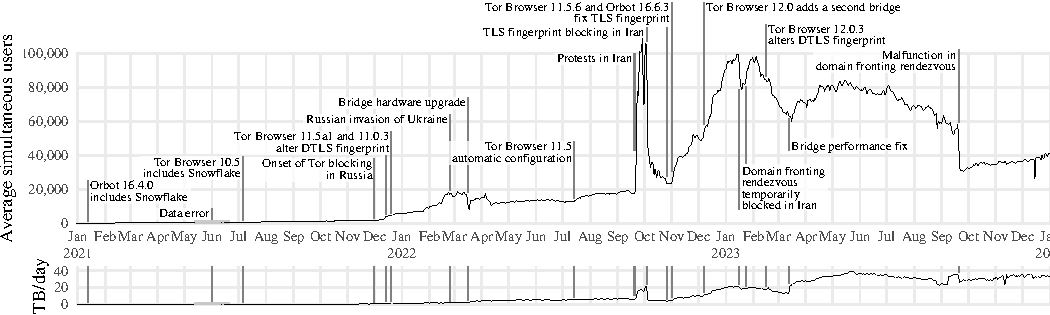
\includegraphics{figures/users/users-global}
\caption{
Estimated average number of simultaneous Snowflake users per day.
The value at the far left,
in early January 2021, is about~60.
% > filter(filtered, abs(date - as.Date("2021-01-01")) < 3)
% # A tibble: 5 x 3
%   date       transport users
%   <date>     <chr>     <dbl>
% 1 2020-12-30 snowflake  66.2
% 2 2020-12-31 snowflake  54.0
% 3 2021-01-01 snowflake  53.4
% 4 2021-01-02 snowflake  65.5
% 5 2021-01-03 snowflake  65.4
At this point, Snowflake was available
for desktop platforms and Android
in Tor Browser's alpha release series,
but not yet in the stable release series.
The maximum value in the part of the graph not shown
is~133, on \mbox{2020-12-09}.
% > filtered[which.max(filter(filtered, date < "2021-01-01")$users), ]
% # A tibble: 1 x 3
%   date       transport users
%   <date>     <chr>     <dbl>
% 1 2020-12-09 snowflake  133.
}
\label{fig:user-counts}
\todo[inline]{Bandwidth chart? Ideally with aligned horizontal axis.}
\todo[inline]{Find a good way to represent the intermittent blocking of the domain front in Iran, January--March~2023.}
\todo[inline]{Pro-rate days with partial coverage (e.g.\ the dip on Feb.~16--17 2023, which was a server restart.}
\end{figure*}

\section{Experience}
\label{sec:experience}

Snowflake has now been operating as a going concern for a few years.
In~lieu of a forward-looking evaluation section
that anticipates how well the system will work in practice,
here we will examine the history of our deployment.

\subsection{Deployment history and user counts}
\label{sec:deployment}

% Excerpts from https://gitlab.torproject.org/tpo/network-health/metrics/timeline:
% |2017-01-24|||snowflake|Tor Browser 7.0a1 released, including Snowflake for GNU/Linux only.|[blog post](https://blog.torproject.org/blog/tor-browser-70a1-released)||
% |2017-08-08|||snowflake|Tor Browser 7.5a4 released, including Snowflake for macOS.|[blog post](https://blog.torproject.org/blog/tor-browser-75a4-released) [issue](https://bugs.torproject.org/tpo/applications/tor-browser/22831)||
% |2018-03-26 20:43:42|||snowflake|Release of Tor Browser 8.0a5. Improves snowflake client performance.|[blog post](https://blog.torproject.org/tor-browser-80a5-released) [ticket](https://bugs.torproject.org/tpo/anti-censorship/pluggable-transports/snowflake/21312)||
% |2019-10-01|||snowflake|Release of Tor Browser 9.0a7, the first release that has Snowflake for Windows.|[blog post](https://blog.torproject.org/new-release-tor-browser-90a7) [ticket](https://bugs.torproject.org/tpo/anti-censorship/pluggable-transports/snowflake/25483)||
% |2020-05-22 19:51:29|||snowflake|Release of Tor Browser 9.5a13, the first release with Turbo Tunnel session persistence features for Snowflake. There is a spike in estimated users on 2020-05-21 and 2020-05-22, which appears to be an artifact.|[blog post](https://blog.torproject.org/new-release-tor-browser-95a13) [ticket](https://bugs.torproject.org/tpo/applications/tor-browser/34043) [users graph](https://metrics.torproject.org/userstats-bridge-transport.html?start=2020-03-01&end=2020-08-01&transport=snowflake)||
% |2020-06-02 18:09:48|||snowflake|Release of Tor Browser 10.0a1, the first release with Snowflake for Android.|[blog post](https://blog.torproject.org/new-release-tor-browser-100a1) [ticket](https://bugs.torproject.org/tpo/applications/tor-browser/30318)||
% |2020-06-25|2020-06-25||snowflake|One- or two-day spike in estimated Snowflake users. It resembles the spike that occurred around the time of the Turbo Tunnel release of Tor Browser 9.5a13 on 2020-05-22.|[users graph](https://metrics.torproject.org/userstats-bridge-transport.html?start=2020-03-01&end=2020-08-01&transport=snowflake)|X|
% |2020-08-19|||snowflake|Release of Tor Browser 10.0a5, which added added the ability to do NAT behavior discovery to the Snowflake client.|[blog post](https://blog.torproject.org/new-release-tor-browser-100a5/) [issue](https://bugs.torproject.org/tpo/applications/tor-browser-build/40016)||
% |2020-10-29|||snowflake|Release of Snowflake WebExtension 0.5.0, with a NAT type self-test.|[archive](https://archive.org/details/snowflake-webextension-0.5.0) [issue](https://bugs.torproject.org/tpo/anti-censorship/pluggable-transports/snowflake/40013)||
% |2020-11-17|||snowflake|Release of Snowflake WebExtension 0.5.2, with a fix to the NAT type self-test.|[archive](https://archive.org/details/snowflake-webextension-0.5.2) [merge request](https://gitlab.torproject.org/tpo/anti-censorship/pluggable-transports/snowflake-webext/-/merge_requests/9) [comment](https://bugs.torproject.org/tpo/anti-censorship/pluggable-transports/snowflake/40013#note_2716071)||
% |2021-01-12|||snowflake|Release of Orbot 16.4.0-RC-1-tor-0.4.4.6, first release with Snowflake client support.|[release](https://github.com/guardianproject/orbot/releases/tag/16.4.0-RC-1-tor-0.4.4.6)||
% |2021-02-23|||snowflake|Release of Orbot 16.4.1-BETA-2-tor.0.4.4.6, with experimental Snowflake proxy support.|[release](https://github.com/guardianproject/orbot/releases/tag/16.4.1-BETA-2-tor.0.4.4.6)||
% |2021-07-06 16:56:37|||snowflake|Release of Tor Browser 10.5, first stable release that includes Snowflake.|[blog post](https://blog.torproject.org/new-release-tor-browser-105)||
% |2021-12-01|ongoing|ru||Blocking of Tor directory authorities, relays, default obfs4 bridges, meek-azure, and Snowflake in some ISPs in Russia. There was a temporary cease of blocking for less than a day starting on 2021-12-08.|[NTC thread](https://ntc.party/t/ooni-reports-of-tor-blocking-in-certain-isps-since-2021-12-01/1477) [BBS thread](https://github.com/net4people/bbs/issues/97) [issue](https://bugs.torproject.org/tpo/community/support/40050) [blog post](https://blog.torproject.org/tor-censorship-in-russia/) [OONI report](https://ooni.org/post/2021-russia-blocks-tor/#blocking-of-the-tor-network)||
% |2021-12-14|||snowflake|Release of Tor Browser 11.5a1, with an altered DTLS fingerprint in Snowflake to counteract blocking in Russia.|[blog post](https://blog.torproject.org/new-release-tor-browser-115a1/) [issue](https://bugs.torproject.org/tpo/applications/tor-browser-build/40393) [NTC post](https://ntc.party/t/ooni-reports-of-tor-blocking-in-certain-isps-since-2021-12-01/1477/59)||
% |2021-12-20|||snowflake|Release of Tor Browser 11.0.3, with an altered DTLS fingerprint in Snowflake to counteract blocking in Russia.|[blog post](https://blog.torproject.org/new-release-tor-browser-1103/) [issue](https://bugs.torproject.org/tpo/applications/tor-browser-build/40393) [NTC post](https://ntc.party/t/ooni-reports-of-tor-blocking-in-certain-isps-since-2021-12-01/1477/59)||
% |2022-01-25 17:41:00|||snowflake|Switched the snowflake bridge to a temporary load-balanced staging server. Debugged connection problems until 2022-01-25 18:47:00.|[issue](https://bugs.torproject.org/tpo/tpa/team/40598#note_2772287) [comment](https://bugs.torproject.org/tpo/anti-censorship/pluggable-transports/snowflake/40095#note_2772325) [post](https://forum.torproject.net/t/tor-relays-how-to-reduce-tor-cpu-load-on-a-single-bridge/1483/16) [comment](https://github.com/net4people/bbs/issues/103#issuecomment-1033067920)||
% |2022-03-16 16:51:35|||snowflake|Moved Snowflake traffic to the interim bridge running instances flakey1–flakey8.|[comment](https://bugs.torproject.org/tpo/tpa/team/40664#note_2787624)||
% |2022-05-06 12:14:51|||snowflake|Upgraded the network uplink of the Snowflake bridge from 1 Gbps to 10 Gbps.|[issue](https://bugs.torproject.org/tpo/anti-censorship/pluggable-transports/snowflake/40138)||
% |2022-06-27|||snowflake|Deployed version 0.6.0 of the Snowflake WebExtension. The main feature added in this release was support for more than one bridge. It had a bug that caused it to stop reporting client IP addresses, which are used for metrics purposes by the bridge.|[archive](https://archive.org/details/snowflake-webextension-0.6.0) [merge request](https://gitlab.torproject.org/tpo/anti-censorship/pluggable-transports/snowflake-webext/-/merge_requests/29) [issue](https://bugs.torproject.org/tpo/anti-censorship/pluggable-transports/snowflake-webext/82)||
% |2022-07-14|||bridge|Release of Tor Browser 11.5, with a new feature of automatic censorship circumvention configuration.|[blog post](https://blog.torproject.org/new-release-tor-browser-115/)||
% |2022-09-21|ongoing|ir||Protests and daily Internet shutdowns in Iran.|[OONI report](https://ooni.org/post/2022-iran-blocks-social-media-mahsa-amini-protests/) [BBS thread](https://github.com/net4people/bbs/issues/125)||
% |2022-10-03 12:50:34|||snowflake|Deployment of Snowflake broker to reject proxies that do not support multiple bridges.|[issue](https://bugs.torproject.org/tpo/anti-censorship/pluggable-transports/snowflake/40193) [issue](https://bugs.torproject.org/tpo/anti-censorship/team/95)||
% |2022-10-04 17:15:00|||snowflake|Snowflake rendezvous blocked by TLS fingerprint in Iran.|[issue](https://bugs.torproject.org/tpo/anti-censorship/pluggable-transports/snowflake/40207) [BBS thread](https://github.com/net4people/bbs/issues/131)||
% |2022-10-12|||snowflake|Release of Tor Browser 11.5.4. Adds uTLS TLS camouflage support for Snowflake, making a manual configuration possible to circumvent recent TLS blocking in Iran.|[blog post](https://blog.torproject.org/new-release-tor-browser-1154/) [BBS comment](https://github.com/net4people/bbs/issues/131#issuecomment-1280391051)||
% |2022-10-17 15:52:00||ir|snowflake|Enabled uTLS for Snowflake in Iran in the Circumvention Settings API, using the `hellochrome_auto` fingerprint.|[comment](https://bugs.torproject.org/tpo/anti-censorship/team/96#note_2844378) [merge request](https://gitlab.torproject.org/tpo/anti-censorship/rdsys-admin/-/merge_requests/6)||
% |2022-10-20 15:16:00|||snowflake|Release of Orbot for Android 16.6.3-BETA-2-tor.0.4.7.10. Adds uTLS TLS camouflage support for Snowflake, making it possible to circumvent recent TLS blocking in Iran.|[release](https://github.com/guardianproject/orbot/releases/tag/16.6.3-BETA-2-tor.0.4.7.10) [announcement](https://github.com/net4people/bbs/issues/125#issuecomment-1285897627)||
% |2022-10-27|||snowflake|Release of Tor Browser 11.5.6. Fixes the problem that prevented Snowflake from working in 11.5.5, and enables uTLS TLS camouflage support by default for Snowflake.|[blog post](https://blog.torproject.org/new-release-tor-browser-1156/) [issue](https://bugs.torproject.org/tpo/applications/tor-browser-build/40665)||
% |2022-11-01||ir|snowflake|Orbot begins a gradual release rollout of version 16.6.3-RC-1-tor.0.4.7.10, which has TLS fingerprint changes to make Snowflake work in Iran again.|[release](https://github.com/guardianproject/orbot/releases/tag/16.6.3-RC-1-tor.0.4.7.10)||
% |2022-12-01|||snowflake|Release of Tor Browser 12.0a5, the first release to contain both the snowflake-01 and snowflake-02 bridges.|[issue](https://bugs.torproject.org/tpo/applications/tor-browser-build/40674) [announcement](https://lists.torproject.org/pipermail/tor-announce/2022-December/000256.html) [BBS comment](https://github.com/net4people/bbs/issues/152#issuecomment-1336220171)||
% |2022-12-07|||snowflake|Release of Tor Browser 12.0, the first stable release to contain both the snowflake-01 and snowflake-02 bridges.|[issue](https://bugs.torproject.org/tpo/applications/tor-browser-build/40674) [blog post](https://blog.torproject.org/new-release-tor-browser-120/) [BBS comment](https://github.com/net4people/bbs/issues/152#issuecomment-1342800169) [NTC comment](https://ntc.party/t/second-snowflake-bridge-available-for-testing/3445/2)||
% |2023-01-16|2023-01-24|ir|moat snowflake|The domain name cdn.sstatic.net, which is used by Snowflake and Moat, is blocked in some ISPs in Iran.|[comment](https://bugs.torproject.org/tpo/anti-censorship/team/115#note_2873040)||
% |2023-01-31|2023-02-01|ir|moat snowflake|The domain name cdn.sstatic.net, which is used by Snowflake and Moat, is again blocked in some ISPs in Iran.|[comment](https://bugs.torproject.org/tpo/anti-censorship/team/115#note_2876012)||
% |2023-02-08|2023-02-13|ir|moat snowflake|The domain name cdn.sstatic.net, which is used by Snowflake and Moat, is again blocked in some ISPs in Iran.|[comment](https://bugs.torproject.org/tpo/anti-censorship/team/115#note_2883298) [OONI chart](https://explorer.ooni.org/chart/mat?probe_cc=IR&since=2023-01-23&until=2023-03-01&time_grain=day&axis_x=measurement_start_day&test_name=web_connectivity&domain=cdn.sstatic.net)||
% |2023-02-15|||snowflake|Release of Tor Browser 12.0.3. Has a change to the Snowflake DTLS fingerprint (removes Hello Verify Request) to mitigate reported blocking in Russia.|[blog post](https://blog.torproject.org/new-release-tor-browser-1203/) [comment about Hello Verify Request](https://bugs.torproject.org/tpo/anti-censorship/censorship-analysis/40030#note_2823140) [Snowflake merge request](https://gitlab.torproject.org/tpo/anti-censorship/pluggable-transports/snowflake/-/merge_requests/134) [Tor Browser merge request](https://gitlab.torproject.org/tpo/applications/tor-browser-build/-/merge_requests/637)||
% |2023-02-19|2023-02-19|ir|moat snowflake|The domain name cdn.sstatic.net, which is used by Snowflake and Moat, is again blocked in some ISPs in Iran.|[comment](https://bugs.torproject.org/tpo/anti-censorship/team/115#note_2883298) [OONI chart](https://explorer.ooni.org/chart/mat?probe_cc=IR&since=2023-01-23&until=2023-03-01&time_grain=day&axis_x=measurement_start_day&test_name=web_connectivity&domain=cdn.sstatic.net)||
% |2023-02-22|2023-02-22|ir|moat snowflake|The domain name cdn.sstatic.net, which is used by Snowflake and Moat, is again blocked in some ISPs in Iran.|[comment](https://bugs.torproject.org/tpo/anti-censorship/team/115#note_2883298) [OONI chart](https://explorer.ooni.org/chart/mat?probe_cc=IR&since=2023-01-23&until=2023-03-01&time_grain=day&axis_x=measurement_start_day&test_name=web_connectivity&domain=cdn.sstatic.net)||
% |2023-03-13 19:46:07|||snowflake|Restarted snowflake-02 bridge for a bugfix.|[comment](https://bugs.torproject.org/tpo/anti-censorship/pluggable-transports/snowflake/40262#note_2886032) [issue](https://bugs.torproject.org/tpo/anti-censorship/pluggable-transports/snowflake/40260)||
% |2023-03-13 20:17:54|||snowflake|Restarted snowflake-01 bridge for a bugfix.|[comment](https://bugs.torproject.org/tpo/anti-censorship/pluggable-transports/snowflake/40262#note_2886041) [issue](https://bugs.torproject.org/tpo/anti-censorship/pluggable-transports/snowflake/40260)||
% |2023-03-15|||snowflake|Release of Orbot for Android v17 BETA 2. First release of Orbot to include the snowflake-02 bridge along with the existing snowflake-01. Has a change to the Snowflake DTLS fingerprint (removes Hello Verify Request) to mitigate reported blocking in Russia.|[release](https://github.com/guardianproject/orbot/releases/tag/17.0.0-BETA-2-tor.0.4.7.11) [Orbot commit adding snowflake-02](https://github.com/guardianproject/orbot/commit/c3f6ee18f17770a5904ad19c3cd24b9c8dcb3885) [IPtProxy commit upgrading Snowflake](https://github.com/tladesignz/IPtProxy/commit/5d0654a6a1439c05d3ee52b2b351b5df1ff3f6dc)||

The deployment of Snowflake to end users was gradual,
reflecting a long development process.
Deployment began in~2017;
however the system only really became usable in~2020,
and began to attract large numbers of users
(enough to merit a censor's attention)
in~2022, following particular generalized
network blocking events in Russia and Iran.
Here we examine the timeline of deployment
and world events,
and their influence on the number of Snowflake users over time.

Snowflake first shipped in the alpha release series of Tor Browser
before graduating to the stable series.
It~first became available for GNU/Linux
with Tor Browser~7.0a1 on \mbox{2017-01-24};
% "First working bundles with Snowflake, for linux only" https://bugs.torproject.org/tpo/anti-censorship/pluggable-transports/snowflake/19001
% "Add snowflake pt to alpha linux builds" https://bugs.torproject.org/tpo/applications/tor-browser/20735
then for macOS
with Tor Browser~7.5a4 on \mbox{2017-08-08}.
% "mac reproducible build" https://bugs.torproject.org/tpo/anti-censorship/pluggable-transports/snowflake/19001
% "[tbb-dev] Please check reproducibility of mac build with Snowflake (e084e83418)" https://lists.torproject.org/pipermail/tbb-dev/2017-July/000579.html
% "Merge Snowflake for mac" https://bugs.torproject.org/tpo/applications/tor-browser/22831
Here we hit a roadblock:
the Chromium-derived WebRTC library we had used to that point
proved difficult to make work in Tor Browser's
cross-compiled and reproducible build environment.
Pion WebRTC~\cite{pion-webrtc} was more suited to our development needs,
and after switching to it we were able to release
Snowflake for Windows
with Tor Browser~9.0a7 on \mbox{2019-10-01}.
% "Android reproducible build of Snowflake" https://bugs.torproject.org/tpo/applications/tor-browser/28672
% "Integrate snowflake into mobile Tor Browser alpha" https://bugs.torproject.org/tpo/applications/tor-browser/30318
Snowflake for Android became available with
Tor Browser~10.0a1 on \mbox{2020-06-02}.

While at this point Snowflake was available
on every platform supported by Tor Browser,
it was not yet comfortably usable.
There were two important parts missing:
no NAT type matching (\autoref{sec:ice})
meant that an assigned proxy was not always compatible with your NAT;
and the lack of persistent session state (\autoref{sec:data-transfer})
meant that even if you were assigned a compatible proxy,
your session would break once that proxy disappeared.
For these reasons, by early 2020,
the average number of concurrent users
had not risen above~40.
% > library("tidyverse")
% > WANTED_FINGERPRINTS <- c(
%     "7659DA0F96B156C322FBFF3ACCC9B9DC01C27C73" = "snowman",
%     "5481936581E23D2D178105D44DB6915AB06BFB7F" = "snowflake-01",
%     "91DA221A149007D0FD9E5515F5786C3DD07E4BB0" = "snowflake-02"
%   )
% > userstats <- read_csv("figures/users/userstats-bridge-transport-multi.csv") %>%
%     filter(transport == "snowflake" & fingerprint %in% names(WANTED_FINGERPRINTS)) %>%
%     mutate(users = users * frac / 100, frac = NULL) %>%
%     group_by(date, transport) %>% summarize(users = sum(users, na.rm = TRUE), .groups = "drop")
%
% Ignoring two apparently anomalous spikes before 2021.
% One on 2020-05-21 and 2020-05-22 (the day of the Turbo Tunnel release):
% > filter(userstats, "2020-05-19" <= date & date <= "2020-05-24")
% # A tibble: 6 x 3
%   date       transport  users
%   <date>     <chr>      <dbl>
% 1 2020-05-19 snowflake   9.16
% 2 2020-05-20 snowflake  13.6
% 3 2020-05-21 snowflake 134.
% 4 2020-05-22 snowflake 388.
% 5 2020-05-23 snowflake   7.9
% 6 2020-05-24 snowflake  13.9
% One on 2020-06-25 and 2020-06-26 (not sure what this one is about):
% > filter(userstats, "2020-06-23" <= date & date <= "2020-06-28")
% # A tibble: 6 x 3
%   date       transport users
%   <date>     <chr>     <dbl>
% 1 2020-06-23 snowflake  17.0
% 2 2020-06-24 snowflake  20.2
% 3 2020-06-25 snowflake  71.7
% 4 2020-06-26 snowflake 211.
% 5 2020-06-27 snowflake  22.5
% 6 2020-06-28 snowflake  33.7
%
% > filtered <- filter(userstats, !(date %in% as.Date(c("2020-05-21", "2020-05-22", "2020-06-25", "2020-06-26"))))
% > filtered[which.max(filter(filtered, date < "2020-05-21")$users), ]
% # A tibble: 1 x 3
%   date       transport users
%   <date>     <chr>     <dbl>
% 1 2020-04-01 snowflake  34.0
The Turbo Tunnel session persistence feature
became available to users in Tor Browser~9.5a13
on \mbox{2020-05-22}.
% "Merge a turbotunnel branch" https://bugs.torproject.org/tpo/anti-censorship/pluggable-transports/snowflake/33745
% "Update snowflake to persist sessions across proxies" https://bugs.torproject.org/tpo/applications/tor-browser/34043
The client part of NAT behavior detection
was released with Tor Browser~10.0a5 on \mbox{2020-08-19},
% "Use STUN to determine NAT behaviour of peers" https://bugs.torproject.org/tpo/anti-censorship/pluggable-transports/snowflake/34129
% "Update snowflake version and prefs to do nat discovery at the client" https://bugs.torproject.org/tpo/applications/tor-browser-build/40016
and the necessary proxy support was released on \mbox{2020-11-17}.
% "Have a remote probe service to test snowflake proxy NAT compatability" https://bugs.torproject.org/tpo/anti-censorship/pluggable-transports/snowflake/40013
% "Wait for ice gathering to complete before probtest" https://gitlab.torproject.org/tpo/anti-censorship/pluggable-transports/snowflake-webext/-/merge_requests/9
% "after merging snowflake-webext!9 (merged), this is finally working" https://bugs.torproject.org/tpo/anti-censorship/pluggable-transports/snowflake/40013#note_2716071
% https://archive.org/details/snowflake-webextension-0.5.2
After this, Snowflake became usable for daily browsing
and the number of users began to grow into~2021.

\autoref{fig:user-counts}
shows the estimated number of Snowflake users since 2021.
As~the bridge in our deployment is a Tor bridge,
we estimate client counts using the ordinary aggregate statistics
collected by the bridge
and the formulas of Tor Metrics~\cite{tor-tr-2012-10-001}.
Tor Metrics graphs are frequently misinterpreted.
Be aware: the chart does not show a count of unique clients,
but rather the \emph{average number of simultaneous clients} per day.
% "The result is an average number of concurrent users, estimated from data collected over a day. We can't say how many distinct users there are."
% https://metrics.torproject.org/reproducible-metrics.html#users
\todo{Can we do better with respect to unique clients? See \href{https://bugs.torproject.org/tpo/network-health/metrics/analysis/40012\#note_2803514}{\#40012}.}
% $ grep '^2022-05-01.*,snowflake,' figures/users/userstats-bridge-transport-multi.csv
% 2022-05-01,5481936581E23D2D178105D44DB6915AB06BFB7F,snowflake,12235.62,100.00
For example, the value of 12,000 on \mbox{2022-05-01}
means that, on average, 12,000 clients were using the service
at any time during the day.
The chart counts clients, not proxies:
a~client's contribution is the same no matter how many
temporary proxies they use over the course of a session.
(See \autoref{fig:proxy-type} instead for a count of proxies,
and \autoref{sec:proxy-churn} for an estimate of how frequently they change.)
The counts should not be taken as exact,
as the formulas involve an estimated parameter~\cite[\S 4]{tor-tr-2012-10-001},
but they are relatively comparable to others
produced by Tor Metrics.
\todo{
Speaking of, should we show Snowflake numbers in context with other PTs and relay users?
% "This graph shows shows all the Tor users in Russia, whether using relays, bridges, or bridges with pluggable transports." https://bugs.torproject.org/tpo/community/support/40050#note_2796770
}

Snowflake's growth began in earnest
when it became part of default installations.
Orbot, a mobile app that provides a VPN-like Tor proxy,
added a Snowflake client in version 16.4.0
on \mbox{2021-01-12}.\todo{Fact-check this date with Guardian Project.}
% 2021-01-12 for v16.4.0-RC-1-tor-0.4.4.6,  according to https://github.com/guardianproject/orbot/releases/tag/16.4.0-RC-1-tor-0.4.4.6
% 2021-01-19 for v16.4.0-RC-1-tor-0.4.4.6,  according to https://www.apkmirror.com/apk/the-tor-project/orbot-proxy-with-tor/orbot-proxy-with-tor-16-4-0-release/
% 2021-01-19 for v16.4.0-RC-2a-tor-0.4.4.6, according to https://www.apkmirror.com/apk/the-tor-project/orbot-proxy-with-tor/orbot-proxy-with-tor-16-4-0-release/
% 2021-02-03 for v16.4.0,                   according to https://mobile.softpedia.com/apk/orbot-proxy-with-tor/
% 2021-02-03 for v16.4.0-RC-2a-tor-0.4.4.6, according to https://apkpure.com/orbot-tor-for-android/org.torproject.android/variant/16.4.0-RC-2a-tor-0.4.4.6-APK
Snowflake became part of the Tor browser stable release series
on \mbox{2021-07-06} in Tor Browser~10.5,
% https://blog.torproject.org/new-release-tor-browser-105
becoming a third built-in circumvention option,
alongside meek and obfs4.
% https://gitlab.torproject.org/tpo/applications/tor-browser-build/-/blob/tbb-10.5-build1/projects/tor-browser/Bundle-Data/PTConfigs/bridge_prefs.js
Being part of the stable series meant that it was
easily to all Tor users,
not only those who had taken the trouble to install a special alpha release.
The number of concurrent users steadily increased
over the next five months,
reaching almost~2,000 by December~2021.

Network blocking events result in sometimes fewer and
sometimes more users of a circumvention system:
fewer if the system has not enough resistance to avoid
itself being caught up in the blocking;
more if remains unblocked and becomes one
among a diminished array of network access options.
Two such censorship events,
one in Russia and one in Iran,
resulted in increases in the number of Snowflake users
by multiples.
(Because they also threatened Snowflake itself in part,
we will have more to say about them in \autoref{sec:challenges}.)

On \mbox{2021-12-01}, a subset of ISPs in Russia suddenly began to block
most forms of access to Tor
including Snowflake~\cite{ooni-2021-russia-blocks-tor}.
(The censor used a feature of the DTLS handshake.)
We released workarounds within a few weeks in
Tor Browser~11.5a1 and~11.0.3,
and in the next two months the total number of users quadrupled,
mostly due to new users in Russia.
The added demand temporarily overwhelmed the bridge hardware;
for a few weeks Snowflake was almost unusably slow.
% "I really want to use snowflake, but it's extremely slow, almost unusable." https://old.reddit.com/r/TOR/comments/t49i14/hello_i_have_a_problem_with_snowflake_can_you/
We~had to invent a new way of deploying a Tor bridge,
using load balancing over multiple processes to permit better scaling;\todo{Cite ``Running a high-performance pluggable transports Tor bridge'' if and when it comes out.}
% https://forum.torproject.net/t/tor-relays-how-to-reduce-tor-cpu-load-on-a-single-bridge/1483
% "The DNS records were changed to point to the staging bridge at..." https://bugs.torproject.org/tpo/anti-censorship/pluggable-transports/snowflake/40095#note_2772325
as well as migrate the bridge to more substantial server hardware
and upgrade from a 1~Gbps to a 10~Gbps network link.
% https://forum.torproject.net/t/tor-project-more-resources-required-for-snowflake-bridge/2353
% "snowflake-01: Change uplink from 1G to 10G" https://bugs.torproject.org/tpo/anti-censorship/pluggable-transports/snowflake/40138
In~May 2022, according to Tor's IP geolocation.
about 70\% of Snowflake users were in Russia.
% > library("tidyverse")
% > WANTED_FINGERPRINTS <- c(
%     "7659DA0F96B156C322FBFF3ACCC9B9DC01C27C73" = "snowman",
%     "5481936581E23D2D178105D44DB6915AB06BFB7F" = "snowflake-01",
%     "91DA221A149007D0FD9E5515F5786C3DD07E4BB0" = "snowflake-02"
%   )
% > userstats <- read_csv("figures/users/userstats-bridge-combined-multi.csv") %>%
%     filter(transport == "snowflake" & fingerprint %in% names(WANTED_FINGERPRINTS)) %>%
%     mutate(across(c(low, high), ~ .x * frac / 100), frac = NULL, users = (pmin(low, high) + high) / 2) %>%
%     # Combine the contributions of all bridges.
%     group_by(date, transport, country) %>% summarize(across(c(low, high, users), sum), .groups = "drop") %>%
%     # Apportion "??" to other countries (see figures/users/users-country.r).
%     group_by(date, transport) %>% mutate(across(c(low, high, users), ~ .x * sum(.x) / sum(ifelse(country == "??", 0, .x)))) %>% ungroup() %>% filter(country != "??")
% > userstats %>% filter(date == "2022-05-20") %>% arrange(desc(users)) %>%
%     mutate(percent = users / sum(users) * 100) %>% head()
% # A tibble: 6 x 7
%   date       transport country   low  high users percent
%   <date>     <chr>     <chr>   <dbl> <dbl> <dbl>   <dbl>
% 1 2022-05-20 snowflake ru      9311. 9311. 9311.   70.4
% 2 2022-05-20 snowflake us      1108. 1109. 1109.    8.38
% 3 2022-05-20 snowflake cn       533.  535.  534.    4.04
% 4 2022-05-20 snowflake de       256.  258.  257.    1.94
% 5 2022-05-20 snowflake by       200.  202.  201.    1.52
% 6 2022-05-20 snowflake gb       184.  186.  185.    1.40
The count of users in Russia get an additional small boost,
visible in the graph,
starting on \mbox{2022-07-14},
when Tor Browser~11.5 added the Connection Assist feature,
which attempts to automatically enable circumvention options when needed.
% https://blog.torproject.org/new-release-tor-browser-115/
% Graph showing boost going mostly to Russia: https://bugs.torproject.org/tpo/anti-censorship/pluggable-transports/snowflake-webext/82#note_2891387
A~separate DTLS blocking signature had been reported on \mbox{2022-06-20};
we did not get to fixing it until Tor Browser~12.0.3 on \mbox{2023-02-15}.\todo{And Orbot 17 on\ldots}
% "The 'skip Hello Verify Request' change was merged into Tor Browser..." https://gitlab.torproject.org/tpo/anti-censorship/censorship-analysis/-/issues/40030#note_2893870
(The apparent one-day dip in the graph on that date is unrelated;
it was a restart of the bridges for a security update.)

% "Shutdowns, intensified blocking in Iran since 2022-09-21" https://github.com/net4people/bbs/issues/125
% "Need to increase number of tor instances on snowflake-01 bridge, increased usage since yesterday [2022-09-21]" https://lists.torproject.org/pipermail/anti-censorship-team/2022-September/000247.html
% "Graphs of user counts from Iran since the onset of shutdowns" https://forum.torproject.net/t/graphs-of-user-counts-from-iran-since-the-onset-of-shutdowns/4843
The second event that had a large effect on Snowflake usage
were nationwide protests in Iran that started on \mbox{2022-09-21},
to which the government responded by imposing periodic network shutdowns
and additional network blocking,
severe even by the standards of a country already notorious
for Internet censorship~\cite{ooni-2022-iran-blocks-social-media-mahsa-amini-protests}.
Internet users in Iran turned to circumvention systems
that continued working despite the new restrictions,
Snowflake among them.
On~\mbox{2022-09-20}, Iran accounted for only~1\% of Snowflake users;
on~\mbox{2022-09-24} it was 67\%.
% > library("tidyverse")
% > WANTED_FINGERPRINTS <- c(
%     "7659DA0F96B156C322FBFF3ACCC9B9DC01C27C73" = "snowman",
%     "5481936581E23D2D178105D44DB6915AB06BFB7F" = "snowflake-01",
%     "91DA221A149007D0FD9E5515F5786C3DD07E4BB0" = "snowflake-02"
%   )
% > userstats <- read_csv("figures/users/userstats-bridge-combined-multi.csv") %>%
%     filter(transport == "snowflake" & fingerprint %in% names(WANTED_FINGERPRINTS)) %>%
%     mutate(across(c(low, high), ~ .x * frac / 100), frac = NULL, users = (pmin(low, high) + high) / 2) %>%
%     # Combine the contributions of all bridges.
%     group_by(date, transport, country) %>% summarize(across(c(low, high, users), sum), .groups = "drop") %>%
%     # Apportion "??" to other countries (see figures/users/users-country.r).
%     group_by(date, transport) %>% mutate(across(c(low, high, users), ~ .x * sum(.x) / sum(ifelse(country == "??", 0, .x)))) %>% ungroup() %>% filter(country != "??")
% > userstats %>% filter("2022-09-19" <= date & date <= "2022-09-25") %>%
%     group_by(date, transport) %>% mutate(percent = users / sum(users) * 100) %>% filter(country == "ir") %>% ungroup()
% # A tibble: 7 x 7
%   date       transport country    low   high  users percent
%   <date>     <chr>     <chr>    <dbl>  <dbl>  <dbl>   <dbl>
% 1 2022-09-19 snowflake ir        205.   207.   206.    1.20
% 2 2022-09-20 snowflake ir        228.   229.   228.    1.32
% 3 2022-09-21 snowflake ir       1023.  1025.  1024.    5.48
% 4 2022-09-22 snowflake ir      17313. 18064. 17691.   51.8
% 5 2022-09-23 snowflake ir      19180. 20037. 19610.   64.7
% 6 2022-09-24 snowflake ir      47469. 49083. 48279.   67.0
% 7 2022-09-25 snowflake ir      45359. 45445. 45445.   67.1
The massive influx of users had us scrambling to test and deploy
performance improvements over the next few days;
the apparent oscillations in this part of the graph
are artifacts caused by our frequently restarting the bridge at this time,
which causes Tor to lose part of a day's metrics.\todo{Reevaluate this after user counts get pro-rated by coverage per day.}
About two weeks later, on \mbox{2022-10-04},
usage dropped as quickly as had risen,
due to the censors in Iran blocking a TLS fingerprint
used for rendezvous.
% "Sudden reduction in snowflake-01 bridge bandwidth, 2022-10-04 17:15" https://bugs.torproject.org/tpo/anti-censorship/pluggable-transports/snowflake/40207
We will have more to say about that in \autoref{sec:block-ir}.
After deploying fixes for the TLS fingerprint issue,
users in Iran began to recover going into~2023.
One of the the emergency performance optimizations we had deployed in late September
turned out to be mistaken and actually be harmful for performance,
% "Weird KCP packets received by the client" https://bugs.torproject.org/tpo/anti-censorship/pluggable-transports/snowflake/40260
though the problem was masked, for a time, by the great demand for the service.
The user count had declined from February~2023,
until we reverted the erroneous change in mid-March,
% "Deploy snowflake-server for QueuePacketConn buffer reuse fix (#40260)" https://bugs.torproject.org/tpo/anti-censorship/pluggable-transports/snowflake/40262
after which the count started to recover.
Around this time, there were also short intervals during which
the domain used for domain-fronting rendezvous
was blocked in some ISPs in Iran,
an evident attempt at blocking that was not sustained.

Through most of this history,
we had run the system's backend bridge on a single server,
upgrading and optimizing it as needed.
Recall from \autoref{sec:mechanics} that it is not a weakness
for the bridge to be a single entity at a well-known address,
because a censor's target of blocking can only be the temporary proxies, not the bridge.
But as the first bridge began to reach its hardware capacity
and performance wins got harder to achieve,
we deployed a second bridge to share the load.
The challenges and design considerations of doing so are discussed in \autoref{sec:multi-bridge}.
The second bridge was made available to users in
Tor Browser~12.0 on \mbox{2022-12-07}.
By~February, however, the second bridge only accounted for about~5\%
of users---evidently the majority of Snowflake users used Orbot
rather than Tor Browser.
\todo{Revisit this when Orbot~17 hits the \href{https://play.google.com/store/apps/details?id=org.torproject.android}{Play Store}}
% > library("tidyverse")
% > WANTED_FINGERPRINTS <- c(
%     "7659DA0F96B156C322FBFF3ACCC9B9DC01C27C73" = "snowman",
%     "5481936581E23D2D178105D44DB6915AB06BFB7F" = "snowflake-01",
%     "91DA221A149007D0FD9E5515F5786C3DD07E4BB0" = "snowflake-02"
%   )
% > userstats <- read_csv("figures/users/userstats-bridge-transport-multi.csv") %>%
%     filter(transport == "snowflake" & fingerprint %in% names(WANTED_FINGERPRINTS)) %>%
%     mutate(users = users * frac / 100, frac = NULL) %>%
%     mutate(instance = WANTED_FINGERPRINTS[fingerprint], fingerprint = NULL) %>%
%     group_by(date, transport) %>% mutate (percent = 100 * users / sum(users, na.rm = TRUE)) %>% ungroup()
% > print(userstats %>% filter("2023-02-20" <= date & date < "2023-02-28"), n = 100)
% # A tibble: 16 x 5
%    date       transport  users instance     percent
%    <date>     <chr>      <dbl> <chr>          <dbl>
%  1 2023-02-20 snowflake 78307. snowflake-01   95.8
%  2 2023-02-20 snowflake  3407. snowflake-02    4.17
%  3 2023-02-21 snowflake 75323. snowflake-01   95.7
%  4 2023-02-21 snowflake  3354. snowflake-02    4.26
%  5 2023-02-22 snowflake 72017. snowflake-01   95.5
%  6 2023-02-22 snowflake  3356. snowflake-02    4.45
%  7 2023-02-23 snowflake 66461. snowflake-01   95.1
%  8 2023-02-23 snowflake  3408. snowflake-02    4.88
%  9 2023-02-24 snowflake 70175. snowflake-01   95.3
% 10 2023-02-24 snowflake  3444. snowflake-02    4.68
% 11 2023-02-25 snowflake 70087. snowflake-01   95.2
% 12 2023-02-25 snowflake  3508. snowflake-02    4.77
% 13 2023-02-26 snowflake 70174. snowflake-01   95.2
% 14 2023-02-26 snowflake  3531. snowflake-02    4.79
% 15 2023-02-27 snowflake 68905. snowflake-01   95.2
% 16 2023-02-27 snowflake  3477. snowflake-02    4.80

As~of \mbox{2023-04-30},
Snowflake had transferred 4.98~PB of user data.\todo{Estimate and subtract non-Snowflake (i.e.~$\langle\mathrm{OR}\rangle$) bytes, even though likely negligible.}
% > library("tidyverse")
% > options(width = 200)
% > WANTED_FINGERPRINTS <- c(
%     "7659DA0F96B156C322FBFF3ACCC9B9DC01C27C73" = "snowman",
%     "5481936581E23D2D178105D44DB6915AB06BFB7F" = "snowflake-01",
%     "91DA221A149007D0FD9E5515F5786C3DD07E4BB0" = "snowflake-02"
%   )
% > read_csv("figures/bandwidth/bandwidth-multi.csv") %>%
%     filter(fingerprint %in% names(WANTED_FINGERPRINTS)) %>%
%     filter(date < "2023-05-01") %>%
%     pivot_wider(names_from = c(type), values_from = c(bytes)) %>%
%     mutate(instance = WANTED_FINGERPRINTS[fingerprint], fingerprint = NULL) %>% relocate(date, instance) %>%
%     # group_by(instance) %>%
%     summarize(date = last(date), across(c(read, write, `dirreq-read`, `dirreq-write`), sum, na.rm = TRUE, .names = "cumul_{.col}")) %>%
%     mutate(
%       cumul_good_read = cumul_read - `cumul_dirreq-read`,
%       cumul_good_write = cumul_write - `cumul_dirreq-write`,
%       cumul_good_avg = (cumul_good_read + cumul_good_write) / 2
%     ) %>%
%     mutate(across(starts_with("cumul_"), scales::label_bytes(units = "auto_si", accuracy = 0.01))) %>%
%     arrange(date)
% # A tibble: 1 x 8
%   date       cumul_read cumul_write `cumul_dirreq-read` `cumul_dirreq-write` cumul_good_read cumul_good_write cumul_good_avg
%   <date>     <chr>      <chr>       <chr>               <chr>                <chr>           <chr>            <chr>
% 1 2023-04-30 5.02 PB    5.05 PB     5.51 TB             94.13 TB             5.01 PB         4.95 PB          4.98 PB
This is goodput; that is, the amount of Tor TLS traffic inside the tunnel.
The bandwidth at the bridges' network interfaces is
higher than the goodput bandwidth,
because of the overhead of WebRTC, WebSocket, and
the internal Turbo Tunnel layer.
At~that time, about 2.7\% of all Tor users
(32\% when looking at just bridge users) used Snowflake to connect to Tor.
\todo{Think about this slight inconsistency: we don't use
\href{https://lists.torproject.org/pipermail/tor-dev/2022-April/014725.html}{\texttt{frac}}
in other estimates/\allowbreak graphs, but here we effectively do.}
% > library("tidyverse")
% > DATE_RANGE <- as.Date(c("2023-04-23", "2023-04-30"))
% > userstats <- bind_rows(
%     read_csv("figures/users/userstats-relay-country.csv", comment = "#") %>%
%       mutate(mode = "relay"),
%     read_csv("figures/users/userstats-bridge-transport.csv", comment = "#") %>%
%       mutate(mode = "bridge")
%   ) %>%
% > filter(lubridate::`%within%`(date, do.call(lubridate::interval, as.list(DATE_RANGE)))) %>%
% > mutate(transport = if_else(mode == "bridge" & transport != "snowflake", "non-snowflake", transport)) %>%
% > group_by(mode, transport) %>% summarize(users = sum(users, na.rm = TRUE), .groups = "drop")
% > userstats %>% mutate(percent = 100 * users / sum(users))
% # A tibble: 3 x 4
%   mode   transport        users percent
% * <chr>  <chr>            <dbl>   <dbl>
% 1 bridge non-snowflake  1464001    5.73
% 2 bridge snowflake       677110    2.65
% 3 relay  NA            23427552   91.6
% > userstats %>% filter(mode == "bridge") %>% mutate(percent = 100 * users / sum(users))
% # A tibble: 2 x 4
%   mode   transport       users percent
%   <chr>  <chr>           <dbl>   <dbl>
% 1 bridge non-snowflake 1464001    68.4
% 2 bridge snowflake      677110    31.6

\subsection{Proxy recruitment and growth}
\label{sec:proxies}

Snowflake's effectiveness depends crucially on its pool of proxies,
of which there are several types.
The primary type is the browser WebExtension,\todo{Audit ``add-on'' vs.\ ``extension'' vs.\ ``WebExtension''.}
% "Creating a Snowflake WebExtension addon" https://bugs.torproject.org/tpo/anti-censorship/pluggable-transports/snowflake/23888
which, once installed, runs the background of a person's web browsing sessions.
There is a ``web badge'' version of the proxy that does not require installation;
it is the same JavaScript code as the WebExtension, but running in a normal web page.
Rather than install a browser extension,
some people leave a browser tab open on a web badge proxy.
There is also a standalone proxy that runs in the command line
and does not require a browser;
% "Golang implementation of standalone snowflake proxy" https://github.com/keroserene/snowflake/pull/41
this version is convenient to install on a rented VPS, for example.
Running a long-term headless snowflake proxy at a fixed IP address
is somewhat at odds with the goal of proxy address diversity,
but these standalone proxy are valuable because
they tend to have less restrictive NATs,
making them compatible with more clients.
Finally, Orbot, a mobile app for accessing Tor,
in addition to being able to \emph{use} a snowflake proxy for circumvention,
can also \emph{provide} snowflake proxy service to others,
a~feature called ``kindness mode.''
% Only so called in Orbot v17+, which should be current by the time the paper is submitted.

\begin{figure}
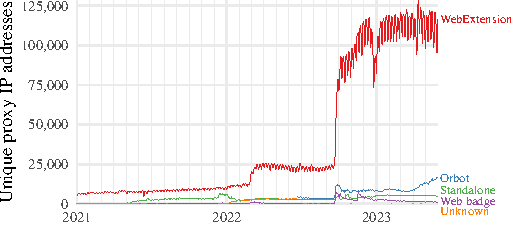
\includegraphics{figures/proxies/proxy-type}
\caption{
Unique proxy IP addresses per day,
by proxy type.
}
\label{fig:proxy-type}
\todo[inline]{Disentangle ``Orbot'' from ``Standalone'' and ``Unknown'' according to known deployment dates.}
% 2021-02-23 https://github.com/guardianproject/orbot/releases/tag/16.4.1-BETA-2-tor.0.4.4.6
% "experimental mode to enable running as a Snowflake proxy"
% 2021-07-14 https://github.com/tladesignz/IPtProxy/commit/228e9e61e285ee548a42d6bee487577e44630695
% IPtProxy 1.1.0 changes its proxy type from "standalone" to "iptproxy"
% 2021-12-20 https://github.com/guardianproject/orbot/releases/tag/16.5.2-RC-1-tor.0.4.6.8
% Orbot updates IPtProxy from 1.0.0 to 1.2.0 https://github.com/guardianproject/orbot/commit/57add48cd904afe94363219887cd142bb5cf6696
% 2022-01-03 https://github.com/guardianproject/orbot/releases/tag/16.5.2-RC-5-tor.0.4.6.9
% This is close to the date (2022-01-05) when there's sudden growth in "Unknown",
% which is probably Orbot self-reporting as "iptproxy" and the broker throwing away that label for being unrecognized.
% 2022-03-21 https://gitlab.torproject.org/tpo/anti-censorship/pluggable-transports/snowflake/-/merge_requests/82
% Broker starts to recognize "iptproxy" as a probe type, but not deployed yet.
% 2022-05-03 https://github.com/tladesignz/IPtProxy/commit/c6ba25ef6ce8449476f734c626eadffdf55d0519
% IPtProxy 1.6.0 adds 'ProxyType: "iptproxy"' (no effective change, had already been done in a patch).
% 2022-06-21 https://bugs.torproject.org/tpo/anti-censorship/pluggable-transports/snowflake/40151
% Broker deployment, broker starts recording "iptproxy" in descriptors.
% 2022-07-05 https://github.com/guardianproject/orbot/releases/tag/16.6.2-RC-1-tor.0.4.7.8
% Orbot 16.6.2 RC 1 upgrades to IPtProxy 1.6.0.
% 2022-08-02 https://github.com/guardianproject/orbot/releases/tag/17.0.0-ALPHA-1-tor.0.4.7.8
% "updated UI based on new design spec: https://github.com/guardianproject/orbot/blob/NEW_UX/docs/design-spec-kindness-mode.md"
% "improved support for Snowflake Proxying "kindness" / volunteer mode"
% 2023-01-13 https://github.com/guardianproject/orbot/releases/tag/17.0.0-BETA-1-tor.0.4.7.11
% "easy access to Snowflake proxy 'kindness' mode"
\end{figure}

\autoref{fig:proxy-type} shows the
comparative counts of the different types of proxy,
counting unique IP addresses per 24~hours.
The WebExtension proxies clearly predominate,
representing about 90\% of daily IP addresses.
% > tail(read_csv("figures/proxies/proxy-type.csv", col_types = cols()) %>% group_by(date) %>% mutate(percent = 100 * unique_ips / sum(unique_ips)) %>% ungroup(), 8)
% # A tibble: 8 x 5
%   date       type       unique_ips coverage percent
%   <date>     <chr>           <dbl>    <dbl>   <dbl>
% 1 2023-04-03 badge           1397.     1       1.07
% 2 2023-04-03 iptproxy        8589.     1       6.57
% 3 2023-04-03 standalone      5084.     1       3.89
% 4 2023-04-03 webext        115652.     1      88.5
% 5 2023-04-04 badge           1009.     0.69    1.11
% 6 2023-04-04 iptproxy        5932.     0.69    6.51
% 7 2023-04-04 standalone      3471.     0.69    3.81
% 8 2023-04-04 webext         80741.     0.69   88.6
The two large steps visible in the graph correspond
to the invasion of Ukraine by Russia in late February~2022,
% 2022-02-25 https://twitter.com/torproject/status/1497276960556429324
% 2022-02-25 https://twitter.com/0xggus/status/1497224413829283877
and protests in Iran beginning late September~2022,
% 2022-09-24 https://twitter.com/torproject/status/1573670895696183303
% 2022-10-03 https://www.eff.org/deeplinks/2022/10/snowflake-makes-it-easy-anyone-fight-censorship
at which times there were campaigns
to encourage people to install the browser extension.

At the outset, it was not clear
that it would be possible to build and sustain
a large enough population of proxies
to be meaningfully blocking resistant
and support a reasonable number of users.
\todo{Give estimated count of flash proxies from
\href{https://people.torproject.org/~dcf/graphs/}{fp-num-proxies-201601.png}.}
% "Start producing snowflakes" https://bugs.torproject.org/tpo/anti-censorship/pluggable-transports/snowflake/20813
While early growth in the number proxies
was due developing new and easier ways to run one,
later growth depended on advocacy and outreach.
In~the early days, circa~2017,
the only round-the-clock proxy support was
a few standalone proxies,
% 2018 "The three fallback proxy-go instances..." https://bugs.torproject.org/tpo/anti-censorship/pluggable-transports/snowflake/25688
run by us for the benefit of alpha testers.
A~page with the web badge existed,
but did not get enough traffic to produce proxies reliably.
The WebExtension was first made available in mid-2019.
% |2019-06-26|||snowflake|Deployed version 0.0.1 of the Snowflake WebExtension for Firefox.|[comment](https://bugs.torproject.org/tpo/anti-censorship/pluggable-transports/snowflake/30931#note_2593598)||
% |2019-07-03|||snowflake|Deployed version 0.0.1 of the Snowflake WebExtension for Chrome.|[comment](https://bugs.torproject.org/tpo/anti-censorship/pluggable-transports/snowflake/30999#note_2593718)||
% |2019-07-26|||flashproxy snowflake|Cupcake 2.0 is released, now working with Snowflake rather than flash proxy.|[Chrome Web Store page](https://chrome.google.com/webstore/detail/cupcake/dajjbehmbnbppjkcnpdkaniapgdppdnc)||
It~got early assistance when Cupcake,
a~browser extension for flash proxy with an existing user base,
% "Link Cupcake from snowflake.torproject.org" https://bugs.torproject.org/tpo/anti-censorship/pluggable-transports/snowflake/31497
% "Snowflake integration" https://github.com/glamrock/cupcake/issues/24
was repurposed for Snowflake, at about the same time.
Orbot's Snowflake proxy feature was added in version 16.4.1 in February~2021,\todo{Check this timing with Guardian Project.}
% 2021-02-23 https://github.com/guardianproject/orbot/releases/tag/16.4.1-BETA-2-tor.0.4.4.6
% https://m.apkpure.com/orbot-tor-for-android/org.torproject.android/download/1641300201-APK has 2021-04-30,
% but I tend to believe the 2021-02-23 because it matches up with features in the graph.
though it was counted with the standalone proxies
until becoming its own proxy type in January~2022.
% 2021-07-14 https://github.com/tladesignz/IPtProxy/commit/228e9e61e285ee548a42d6bee487577e44630695
% IPtProxy 1.1.0 changes its proxy type from "standalone" to "iptproxy"
% 2021-12-20 https://github.com/guardianproject/orbot/releases/tag/16.5.2-RC-1-tor.0.4.6.8
% Orbot updates IPtProxy from 1.0.0 to 1.2.0 https://github.com/guardianproject/orbot/commit/57add48cd904afe94363219887cd142bb5cf6696
% 2022-01-03 https://github.com/guardianproject/orbot/releases/tag/16.5.2-RC-5-tor.0.4.6.9
% Changes from "standalone" to "unknown" because the broker does not recognize "iptproxy".
% 2022-06-21 https://bugs.torproject.org/tpo/anti-censorship/pluggable-transports/snowflake/40151
% Broker deployment, starts recognizing "iptproxy".

\todo{Compare the number of Snowflake proxies with the
\href{https://metrics.torproject.org/networksize.html}{number of other kinds of bridges}.
Caveat: the other bridges have supposedly better anti-enumeration defenses.}

It~is worth reflecting briefly
on the relative ineffectiveness of the web badge
compared to the WebExtension.
The web badge had been the primary envisioned deployment model of flash proxy
(though by the end of its run, flash proxy had also gained
% https://www.bamsoftware.com/talks/ee380-flashproxy/index.html#s15
browser extensions including Cupcake
% "Chrome browser add-on" [Cupcake for flash proxy] https://bugs.torproject.org/legacy/trac/7721
% "Tor Flashproxy Badge" [for Firefox] https://github.com/reezer/tor-flashproxy-badge/
and a standalone proxy,
% "Node.js standalone flash proxy" https://bugs.torproject.org/legacy/trac/7944
much like Snowflake later would).
The idea had been that people's browsers
would automatically become proxies
while they browsed sites that had the flash proxy code installed,
unless they had checked an option to prevent~it.
We decided, early on, that flash proxy's opt-out model had been a mistake,
% Date: Tue, 6 Dec 2016 18:38:40 -0800
% From: David Fifield <dcf@torproject.org>
% To: Arlo Breault <arlo@torproject.org>
% Cc: Serene <serene@torproject.org>
% Subject: Re: Snowing
% Message-ID: <20161207023840.mli4cymr6s3aanpu@happy.bamsoftware.com>
%
% My original plan was to repurpose existing flash proxy badges as
% Snowflake badges. But, I am thinking more and more that Snowflake should
% use an opt-in model, rather than opt-out. The opt-out model of flash
% proxy always bothered me. I think there's a good chance it would cause
% trouble for us if Snowflake becomes popular. So I'd like to see
% Snowflake use opt-in badges (and Cupcake) only.
and that Snowflake would be only opt-in:
before becoming a proxy, a person would have to take a positive action
such as installing a browser extension
or activating a toggle on a web page.
% "Prepare a Snowflake 'options' page, like in flashproxy" https://github.com/keroserene/snowflake/issues/21
Our initial concerns that this decision
would reduce the number of proxies were unfounded:
people find an informative, interactable proxy control panel more appealing,
and install the WebExtension in greater numbers.
The browser-based proxies display the number of censored clients
helped in the last 24~hours,
which proxy operators find rewarding.

\subsection{Proxy churn}
\label{sec:proxy-churn}

% https://bugs.torproject.org/tpo/anti-censorship/pluggable-transports/snowflake/34075
% https://gitlab.torproject.org/tpo/anti-censorship/pluggable-transports/snowflake/-/merge_requests/95

The size of the proxy pool is not the only measure of its quality.
Also important is its ``churn,'' the rate at which
one proxy in the pool is replaced by another.
Churn indicates how hard a censor would have to work
to keep a proxy block list up to date;
or conversely,
how quickly even a momentarily complete block list
would lose effectiveness.

We ran an experiment to measure churn.
Every hour, the broker logged a record representing
the proxy IP addresses it had seen in the past hour.
To~avoid the need to store, and risk exposing, real proxy IP addresses,
each record was not a plain list of addresses,
but a HyperLogLog++ sketch~\cite{Heule2013a},
a~probabilistic data structure for estimating
the number of distinct elements in a multiset.
We additionally hashed proxy IP addresses with a consistent secret string,
to prevent the recovery of past proxy IP addresses from our published data.
A~sketch supports two basic operations: count and merge.
Given a sketch~\(X\),
we may compute an approximate count \(|X|\)
of its unique elements;
given two sketches \(X\) and~\(Y\),
we may merge them into a new sketch
that represents their union \(X \cup Y\).
What we are really interested in is the intersection
of two sketches, which may be computed using the formula
\(|X| + |Y| - |X \cup Y|\).
For us, the intersection represents
how many IP addresses are the same
in the proxy pool at two different points in time.

\begin{figure}
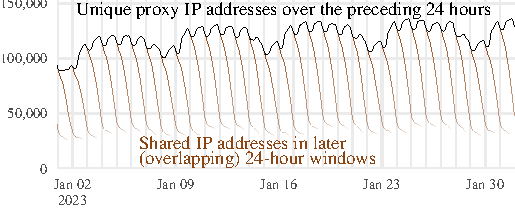
\includegraphics{figures/proxy-churn/proxy-count-decay}
\caption{
Proxy pool churn in January 2023.
The dark upper line shows the number
of unique proxy IP addresses in overlapping 24-hour windows,
sampled at intervals of 1~hour.
The descending lines show
how many of the same IP addresses remain the pool,
at 1-hour intervals up to 40 hours later.
It~takes about 20~hours for 50\% of the proxy pool to turn over.
}
\label{fig:proxy-count-decay}
\end{figure}

\autoref{fig:proxy-count-decay}
visualizes churn according to our proxy pool measurements.
We merged consecutive sketches over a 24-hour window
to serve as a reference,
then computed the size of its intersection
with other windows of the same size,
offset by \(+1, +2, \ldots, +40\) hours.
After 1~hour, the shifted window still has, on average,
97.3\% of addresses in common with the reference;
after 12~hours the fraction has fallen to 68.8\%;
by the time 24~hours have elapsed,
38.2\% of proxy IP addresses
are ones that had been seen in the previous day.
% > library("tidyverse")
% > options(width = 200)
% > DATE_RANGE <- as.Date(c("2023-01-01", "2023-02-01"))
% > read_csv("figures/proxy-churn/proxy-churn-windows.csv") %>%
%     filter(lubridate::`%within%`(reference_timestamp_end, do.call(lubridate::interval, as.list(DATE_RANGE)))) %>%
%     mutate(
%       sample_offset_hours = round(sample_timestamp_end_offset / 3600),
%       intersection_count = reference_count + sample_count - union_count
%     ) %>%
%     group_by(sample_offset_hours) %>%
%     summarize(
%       across(c(reference_count, sample_count, union_count, intersection_count), mean),
%       intersection_percent = 100 * intersection_count / reference_count,
%       .groups = "drop"
%     ) %>%
%     filter(sample_offset_hours %in% c(0, 1, 2, 3, 4, 8, 12, 18, 24, 36, 40))
% # A tibble: 11 x 6
%    sample_offset_hours reference_count sample_count union_count intersection_count intersection_percent
%                  <dbl>           <dbl>        <dbl>       <dbl>              <dbl>                <dbl>
%  1                   0         119654.      119654.     119654.            119654.                100
%  2                   1         119654.      119704.     122907.            116450.                 97.3
%  3                   2         119654.      119754.     126142.            113266.                 94.7
%  4                   3         119654.      119804.     129359.            110099.                 92.0
%  5                   4         119654.      119854.     132529.            106980.                 89.4
%  6                   8         119654.      120060.     145141.             94572.                 79.0
%  7                  12         119654.      120292.     157684.             82262.                 68.8
%  8                  18         119654.      120649.     176400.             63903.                 53.4
%  9                  24         119654.      120970.     194892.             45732.                 38.2
% 10                  36         119654.      121500.     206542.             34612.                 28.9
% 11                  40         119654.      121639.     208269.             33024.                 27.6

\subsection{Development challenges}
\label{sec:challenges}

Designing a circumvention system in the abstract,
and building it out into something that is practical and useful,
present different sets of challenges---and
the latter are no less important than the former.
Besides the obvious need
to continually check design assumptions
against the actual behavior of censors,
there are all sorts of considerations around
managing development complexity,
deploying on multiple platforms,
and administering servers.
While seemingly mundane, they can mean the difference between success and failure.
% "Under this understanding of censorship as friction, the usability of circumvention tools becomes even more important." https://github.com/net4people/bbs/issues/122#issuecomment-1232334948

The primary make-or-break challenge was finding a way to make
WebRTC, a suite of protocols of and for the web,
usable outside the browser,
in order to make a general-purpose proxy capable of transmitting
not just web, but Tor and any other traffic.
In~2016 there were not as many options as there are now.
Our own \mbox{go-webrtc} package,
which extracted the C++ WebRTC library
from the Chromium web browser and added bindings
for the Go programming language,
was one of the early efforts in this area and indeed,
a~key ingredient without which
the Snowflake project could not have gotten started.
But having Chromium as a critical dependency proved troublesome.
Chromium is a large, complex piece of software
with a custom and frequently changing build system.
Every update was an ordeal.
% 2016-06-06 "Play catch up w/ upstream" https://github.com/keroserene/go-webrtc/issues/39
% 2016-06-22 "Bump to branch-heads/52" https://github.com/keroserene/go-webrtc/pull/42
% 2016-09-23 "GN migration" https://bugs.torproject.org/tpo/anti-censorship/pluggable-transports/snowflake/19001#note_2591236
% 2017-06-06 "libwebrtc and snowflake are not being built reproducibly (unless you build in the same month)" https://bugs.torproject.org/tpo/applications/tor-browser/22832
% 2017-11-28 "Snowflake broken if no libatomic on host" https://bugs.torproject.org/tpo/applications/tor-browser/24465
% 2017-03-13 "Update to branch-head/58 and add ARM support." https://github.com/keroserene/go-webrtc/pull/61
% 2017-04-15 "Snowflake breaks the 7.0a3 build" https://bugs.torproject.org/tpo/anti-censorship/pluggable-transports/snowflake/21954
% 2018-03-29 "Update to branch-heads/64" https://github.com/keroserene/go-webrtc/pull/79
% 2018-04-03 "Figure out something for CI so we don't have to build w/ -D_GLIBCXX_USE_CXX11_ABI=0" https://github.com/keroserene/go-webrtc/issues/81
% 2018-05-31 "Adapt macOS snowflake compilation to new toolchain" https://bugs.torproject.org/tpo/applications/tor-browser/26251
% 2018-12-07 "Assembling WebRTC sources fails with error 'You have unstaged changes'" https://bugs.torproject.org/tpo/applications/tor-browser/28784
% 2019-08-06 "Provide support for v21 SCTP offer spec" https://github.com/keroserene/go-webrtc/issues/107
It~was the kind of thing
a large team of web browser build engineers could keep up with,
but not a small team of circumvention developers.
Tor Browser requires that all its software components
build reproducibly from source,
in a cross-compiling environment without any
pre-built or proprietary dependencies.
Despite extensive hacking,
we were never able to make a Windows build
work in this environment---and
% "windows reproducible build" https://bugs.torproject.org/tpo/anti-censorship/pluggable-transports/snowflake/19001#note_2591246
% "Windows reproducible build of snowflake" https://bugs.torproject.org/tpo/anti-censorship/pluggable-transports/snowflake/25483
% 2015-12-22 "native webrtc dependency build script" https://github.com/keroserene/go-webrtc/issues/23
% 2016-02-02 "[WIP] Script to build-from-scratch from upstream webrtc" https://github.com/keroserene/go-webrtc/pull/32
% 2017-01-04 "libwebrtc-magic.a equivalent file for windows machine" https://github.com/keroserene/go-webrtc/issues/57
% 2017-10-02 "I put in all the work to get DLL linkage in" https://github.com/keroserene/go-webrtc/pull/69
% 2018-04-06 "How to run latest commit with Windows? (branch-heads/64)" https://github.com/keroserene/go-webrtc/issues/83
not working on Windows is surely a damper on usability.
% (Chromium did not have even basic support for cross-compiling for Windows until late in 2017.)
% https://groups.google.com/a/chromium.org/g/chromium-dev/c/cIA9fBb9vBE/m/73cOvZu9BQAJ
% https://chromium.googlesource.com/chromium/src/+log/e9464b64f5f8cb3ff66965e16c16bec2648910fc/docs/win_cross.md
What finally broke through the impasse was a switch
% "Consider Native WebRTC Implementation" https://github.com/keroserene/go-webrtc/issues/26
% "Evaluate pion WebRTC" https://bugs.torproject.org/tpo/anti-censorship/pluggable-transports/snowflake/28942
to Pion WebRTC~\cite{pion-webrtc} in~2019.
Pion is an independent implementation WebRTC,
written in Go like Snowflake itself,
and easily cross-compilable.
While Pion's not being based on browser code
gives rise to more fingerprinting concerns
of the kind discussed in \autoref{sec:fingerprinting},
the time and attention it has freed up
has been more than worth~it.
% A few more libwebrtc problems:
% "Memory and file descriptor leaks in programs that use go-webrtc" https://bugs.torproject.org/tpo/anti-censorship/pluggable-transports/snowflake/21312
% "Bump snowflake/go-webrtc for trac 21312" https://bugs.torproject.org/tpo/applications/tor-browser/25449
% "Bump snowflake/go-webrtc again for trac 21312" https://bugs.torproject.org/tpo/applications/tor-browser/25579
% 2019-05-03 "Any go program that uses this library will have an executable stack..." https://github.com/keroserene/go-webrtc/pull/105

% History of changing domain fronts
% 2017-06-10 "Standalone broker (independent of App Engine)" https://bugs.torproject.org/tpo/anti-censorship/pluggable-transports/snowflake/22874
% 2018-04-13 "Domain fronting to App Engine stopped working" https://bugs.torproject.org/tpo/anti-censorship/pluggable-transports/snowflake/25804
% 2018-05-02 "Change Snowflake rendezvous to use Azure" https://bugs.torproject.org/tpo/applications/tor-browser/26010
% 2018-05-03 "Additional domain fronts for Snowflake rendezvous" [switch to Azure] https://bugs.torproject.org/tpo/anti-censorship/pluggable-transports/snowflake/22782#note_2591690
% 2021-04-05 "Switch front domain and host to fastly" https://gitlab.torproject.org/tpo/anti-censorship/pluggable-transports/snowflake/-/merge_requests/33
% 2021-08-13 "Is there a better moat/snowflake SNI than cdn.sstatic.net?" https://bugs.torproject.org/tpo/anti-censorship/pluggable-transports/snowflake/40068

The fact that snowflake proxies run in a web browser
is the source of some confusion:
do I~install the browser extension if I~am censored,
or if I~want to help someone else who is censored?
% https://apps.apple.com/us/app/torproject-snowflake/id1597501940
% "Snowflake bridges do work in Iran but only in official Tor bundle. It'll be great if the developers get this extension to work for Iranian users."
The true situation is of course the latter,
but it is natural for a user to assume
that a circumvention-related browser extension is something
they can use to unblock their own connection.
This confusion is probably the cause of
the relatively large proportion of \emph{proxies} in Iran
(about 5\% of unique IP addresses in April~2023).
% tail(read_csv("figures/proxies/proxy-country.csv", col_types = cols()) %>% group_by(date) %>% mutate(percent = 100 * unique_ips / sum(unique_ips)) %>% ungroup() %>% arrange(date, unique_ips) %>% filter(date == "2023-04-15"), 5)
% # A tibble: 5 x 5
%   date       country unique_ips coverage percent
%   <date>     <chr>        <dbl>    <dbl>   <dbl>
% 1 2023-04-15 gb           3042.        1    2.43
% 2 2023-04-15 ca           3976.        1    3.18
% 3 2023-04-15 ir           6312.        1    5.05
% 4 2023-04-15 us          18903.        1   15.1
% 5 2023-04-15 de          54553.        1   43.6
There is similar confusion possible with Orbot,
which has options both
to \emph{use} a proxy and to \emph{be} a proxy.

The Snowflake system
admittedly contains a lot of moving parts.
It~is, unfortunately,
something that requires a team to manage---it
cannot easily be deployed by an individual for their own use,
as some other systems can.
Some complexity is inherent in its nature:
Snowflake is more complicated than a one-hop proxy
and always will be.
Complexity is the enemy of security and robustness, however,
and in a system meant for real production use
could even be considered an existential risk,
if the demands of maintenance exceed what the maintainers can provide.
Managing complexity and designing for low maintenance
are material concerns,
and must sometimes take priority over
development of new features or performance optimization.

% Safe Browsing / zip bomb problem (2019)
% https://bugs.torproject.org/tpo/anti-censorship/pluggable-transports/snowflake/31250

\subsection{Multiple bridges}
\label{sec:multi-bridge}

% "Prepare all pieces of the snowflake pipeline for a second snowflake bridge" https://bugs.torproject.org/tpo/anti-censorship/pluggable-transports/snowflake/28651
% "Distributed Snowflake Server Support" https://bugs.torproject.org/tpo/anti-censorship/pluggable-transports/snowflake/40129
% Ancient history from flash proxy: "allow the client to pick a specific relay for its registration" https://bugs.torproject.org/legacy/trac/10196

The bridge in the Snowflake model (\autoref{sec:mechanics})
is notionally a single, centralized entity.
It~\emph{can} be centralized
because it is insulated from direct blocking
by the snowflake proxies.
Unlike traditional proxy systems,
Snowflake does not benefit, in terms of blocking resistance,
by having multiple bridges,
since the bridge is decoupled from the means of accessing it.
For practical performance reasons, though,
it makes sense for ``the'' bridge to be realized as
multiple servers, simply because the load of Snowflake traffic
is a lot for one server to handle.
\todo{Note fraction of total Tor traffic.}
For technical reasons, though,
the use of multiple bridges cannot be made fully transparent to clients
without making some compromises.
One of the reasons, relatively minor, is related to Snowflake itself;
the other, more constraining one has to do with its interaction with Tor.
We will explain the tradeoffs involved
and the design we settled on.

What is called the bridge is actually a pipeline of several components.
One component terminates incoming WebSocket connections arriving from proxies,
one decodes the Turbo Tunnel packets contained therein and reassembles them into streams,
and one forwards the streams to their eventual destinations
(in~our deployment, this last component is Tor itself).
These components are separable.
For example, because the interface with Tor is ordinary TCP sockets,
it is easy to run Tor on a different host with its own CPU and RAM,
% A diagram of such separation: https://bugs.torproject.org/tpo/anti-censorship/pluggable-transports/snowflake/28651#note_2783541
or even round-robin over multiple instances of Tor
(as we do\todo{Cite ``Running a high-performance pluggable transports Tor bridge''.}).

What is not so easy to distribute
is the Turbo Tunnel layer itself.
Recall from \autoref{sec:data-transfer} that Snowflake
has a notion of a long-term end-to-end session
between the client and the bridge that is independent of
the temporary proxies in between.
This is made possible by extensive state stored at the bridge:
a table of ongoing sessions, reassembly buffers,
transmission queues, timers, and so on.
% `type KCP` https://github.com/xtaci/kcp-go/blob/03b584b84eddd95cc03dbff65fc9cc5cbdf80c6b/kcp.go#L132
% `type UDPSession` https://github.com/xtaci/kcp-go/blob/03b584b84eddd95cc03dbff65fc9cc5cbdf80c6b/sess.go#L61
While it is certainly possible to instantiate more than one such state machine,
a~session that is begun in one instance must remain in that instance---any
other instance will not have the state necessary to make the packets
of the session meaningful.

The other difficulty is a Tor bridge is identified
by a \firstterm{bridge fingerprint},
a hash of its long-term Tor identity key.
The bridge configuration interface in the Tor client
expects a bridge fingerprint,
and if the bridge it connects to cannot prove that
its identity matches that fingerprint,
the client will terminate the connection~\cite[\S 5.1.2]{tor-spec}\todo{Verify that this is the relevant section of the spec.}.
% https://gitweb.torproject.org/torspec.git/tree/tor-spec.txt?id=33308845cec54bfc0096b8ea0339a8ff183aa1b1#n1153
% "Extending ORs MUST check _all_ provided identity keys (if they recognize the format), and and MUST NOT extend the circuit if the target OR did not prove its ownership of any such identity key."
There is no facility in Tor for a certificate,
or anything like that,
to authorize a whole set of equivalent bridge fingerprints:
the fingerprint of every bridge a client may use
must be configured separately at the client.
While it is possible to copy identity keys between
separate instances of Tor so they have the same fingerprint,
and desirable to do so within one bridge installation for performance reasons,
our vision for scaling the Snowflake backend
involved bridge sites in different locations,
managed by different teams,
and we decided that we did not want the trust boundary
of who has access to those important keys to be quite so large.

In short, the client must know in advance which bridge
its snowflake proxy will connect (or re-connect) it to.
If~the first connection is to a bridge other than the one the client expects,
the Tor client will abandon the connection because the bridge fingerprint is wrong.
Subsequent re-connections in the same client session
need to go to the same bridge,
otherwise the Turbo Tunnel session state will be missing.

These considerations led us to a multi-bridge design
in which the client has awareness of (at least a subset of)
all the bridges that exist,
and it is the client that chooses which bridge will be used
for a particular session.
The client includes a bridge fingerprint
in its rendezvous message (\autoref{sec:rendezvous}) to the broker;
the broker maps the fingerprint to a WebSocket URL,
and conveys that URL to the proxy.
We~rely on clients choosing uniformly
to equalize the load across bridges.
A~consequence is that
every bridge must meet some minimum performance standard:
we cannot, say,
assign 20\% of clients to one and 80\% to another
according to their relative capabilities.
A~further drawback is that there is no way to try connecting
to only one of the bridges it knows about,
short of rewriting the configuration file;
if two bridges are configured, Tor will start two sessions through Snowflake,
each doing its own independent rendezvous,
which is wasteful and makes the network fingerprint more conspicuous.
% "Let bridge users choose to only reach their first working bridge" https://bugs.torproject.org/tpo/core/tor/40578
Still, this is the best solution we have found, given the limitations.
A~deployment not based on Tor would have more flexibility here.
The only consideration would be the Turbo Tunnel session state,
which could be solved by hashing a client's session identifier string
to consistently assign the same bridge during a session.

A~client-chooses design risks the possibility
of misuse by clients, if not handled carefully.
The client should be able to select
a proxy destination from the set of known bridges,
but not cause a proxy to connect to arbitrary destinations,
otherwise the many proxies of \autoref{sec:proxies}
could be used to attack third parties.
% "Clients cannot cause a proxy to attack or even connect to an arbitrary web site or relay..." https://forum.torproject.net/t/anyone-experiencing-problems-with-snowflake-proxy/6938/15
% An alternative vision: "(More) Distributed servers" https://bugs.torproject.org/tpo/anti-censorship/pluggable-transports/snowflake/40248
When the client expresses its bridge selection
in its rendezvous message, the selection is represented
not as an IP address or domain name,
but as a bridge fingerprint (a~\mbox{40-digit} hexadecimal string).
The broker maps the fingerprint to a WebSocket URL
by consulting a local database of known Snowflake bridges.
The broker rejects client rendezvous messages requesting an unknown fingerprint.
% https://gitlab.torproject.org/tpo/anti-censorship/pluggable-transports/snowflake/-/blob/8e5ea8261110e97a8df56cfc9c83028081d902fb/broker/ipc.go#L187
The broker then tells an incoming proxy
what WebSocket URL to connect this particular client to,
% https://gitlab.torproject.org/tpo/anti-censorship/pluggable-transports/snowflake/-/blob/8e5ea8261110e97a8df56cfc9c83028081d902fb/broker/ipc.go#L144
but here also there is a check.
Proxies check the hostname of the URLs
to ensure that it is a subdomain of a known suffix reserved for Snowflake bridges.
So~there are two independent safeguards against misuse.

As~of May 2023\todo{Update on publication.},
there are two Snowflake bridges,
which are among the largest relays in the Tor network,
in terms of bandwidth.\todo{Do some analysis from figures/\allowbreak onionoo.}
% Actually head-and-shoulders the largest relays?
% figures/onionoo$ jq -r '(.relays+.bridges)|sort_by(-.advertised_bandwidth)[]|[.nickname,.advertised_bandwidth]|@tsv' top-consensus_weight.onionoo.json | head -n 4
% RandomRecipes	114341160
% poiuty	109014582
% xor	103805661
% StayStrongRelay01	99326969
% figures/onionoo$ jq -r '(.relays+.bridges)|sort_by(-.advertised_bandwidth)[]|[.nickname,.advertised_bandwidth*12]|@tsv' snowflake-??.onionoo.json
% flakey6	467165892
% crusty7	178083996

% https://archive.is/aYyxR 2023-04-29 archive of https://metrics.torproject.org/rs.html#toprelays
% https://archive.is/zOp4G 2023-04-29 archive of https://metrics.torproject.org/rs.html#aggregate/as
% https://archive.is/GHBKE 2023-04-29 archive of https://metrics.torproject.org/rs.html#details/5481936581E23D2D178105D44DB6915AB06BFB7F (snowflake-01) (multiply by 12)
% https://archive.is/LKFxo 2023-04-29 archive of https://metrics.torproject.org/rs.html#details/91DA221A149007D0FD9E5515F5786C3DD07E4BB0 (snowflake-02) (multiply by 12)
% Relay bandwidth aggregated by AS: https://metrics.torproject.org/rs.html#aggregate/as; on 2023-04-29 Snowflake bridges provide about as much advertised bandwidth as Emerald Onion.

% \subsection{SQL injection attempts at broker}
% \url{https://bugs.torproject.org/tpo/anti-censorship/pluggable-transports/snowflake/40089}
% Actually tailored to the broker protocol, not a generic attack tool.

\section{Notable blocking attempts}
\label{sec:block}

We have seen Snowflake's user counts in \autoref{sec:deployment},
and remarked on how they have at times been affected by blocking actions by censors.
Now we take a closer look at the technical details of specific censorship events.
The effect of these has usually been rather to increase rather than decrease
the number of Snowflake users.
Though seemingly paradoxical, this effect is easy to explain:
as the intensity of censorship increases,
users are displaced from less resilient systems
to more resilient systems.
Snowflake's blocking resistance has not in every case been an unqualified success,
though, and here we also reflect on missteps
and persistent challenges.

The examples are taken from
Russia, Iran, and Turkmenistan,
and are selected for being significant and instructive.
Common themes are that having a line of communication
with affected users is invaluable in understanding and reacting to blocking;
and that a circumvention system's blocking resistance
can only be understood in relation to a censor,
because every censor's cost calculus is different.

Snowflake is blockable by any censor that is willing to block all WebRTC.
We~would not try to claim otherwise.
Indeed, we believe that that is the way circumvention systems
should be presented:
not to argue their unblockability in universal terms,
but by specifying, as completely as possible,
what actions by the censor would suffice to block it---or
more to the point,
\emph{what sacrifices a censor would have to make}
in order to block~it.
Some censors may be able to make those sacrifices; others may not.
Advancing the state of the art in censorship circumvention
consists of finding techniques that put blocking
farther out of reach of would-be controllers of information.
\todo{Reflect on a good location to place this sentiment.}

\begin{figure}[t!]
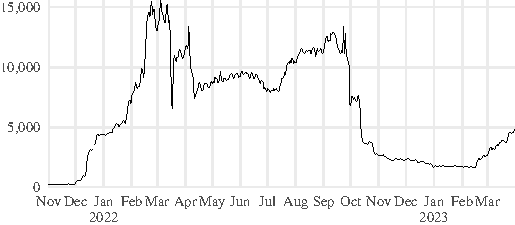
\includegraphics{figures/users/users-ru}
\caption{
Snowflake users in Russia.
The blocking of Tor-related transports in December~2021
led to Snowflake's first surge in usage.
The decrease in September~2022
coincided with an even larger influx of users from Iran,
which may have masked another blocking rule.
}
\label{fig:user-counts-ru}
\bigskip
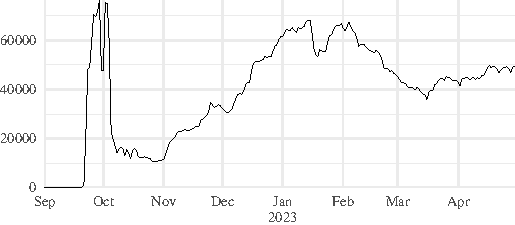
\includegraphics{figures/users/users-ir}
\caption{
Iran.
}
\label{fig:user-counts-ir}
\bigskip
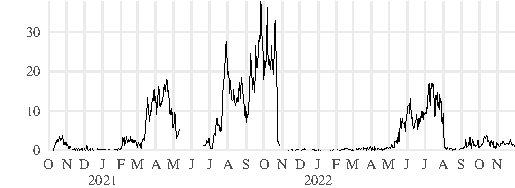
\includegraphics{figures/users/users-tm}
\caption{
Turkmenistan.
}
\label{fig:user-counts-tm}
\todo[inline]{Add annotations for specific events, like \autoref{fig:user-counts}.}
\end{figure}

\subsection{Blocking in Russia}
\label{sec:block-ru}

% "[Russia] Some ISPs are blocking Tor" https://bugs.torproject.org/tpo/community/support/40050
% "OONI reports of Tor blocking in certain ISPs since 2021-12-01" https://ntc.party/t/ooni-reports-of-tor-blocking-in-certain-isps-since-2021-12-01/1477
% "Responding to Tor censorship in Russia" https://blog.torproject.org/tor-censorship-in-russia/

Snowflake, along with other common ways of accessing Tor,
was blocked in a subset of ISPs in Russia
% https://ntc.party/t/ooni-reports-of-tor-blocking-in-certain-isps-since-2021-12-01/1477/95
% "Tor filtering is done using government black box called TSPU.
% Not all providers have them. Tor is not blocked if TSPU is not present.
% According to tor metrics graph directly connecting users decreased only by 1/3.
% This indicates TSPU is not everywhere."
\todo{Consider introducing TSPU? Or not?}
on \mbox{2021-12-01}~\cite{ooni-2021-russia-blocks-tor}.
The blocking action was clearly pre-planned and targeted,
as it happened suddenly and affected multiple Tor-related protocols.
Besides Snowflake,
the IP addresses of a portion
of unobfuscated Tor relays and bridges,
as well as some servers of
the blocking-resistant transports meek and obfs4,
were blocked, at least temporarily.
As~you might expect, the attempt to block
various blocking-resilient transports
was less than totally successful,
and the ultimate effect was a substantial increase in the number
of users accessing Tor via circumvention transports,
Snowflake among them---see the left side of \autoref{fig:user-counts-ru}.
% "A zoom on just the bridge transports" https://bugs.torproject.org/tpo/community/support/40050#note_2796770
% That pluggable transports could not compensate fully
% for the loss of relay users points to a usability gap.
For an overview of how Tor-related transports were affected at this time,
see an article by Ramesh, Sundara Raman, et~al.~\cite[\S 6.2]{Ramesh2023a}.
Here, our focus is on Snowflake.

We~had the benefit of established relationships
and communication with developers and users in Russia,
one of whom, through manual tests, was able to
isolate the traffic feature used to distinguish Snowflake.
It~was DTLS fingerprinting,
of the kind cautioned about in \autoref{sec:fingerprinting}.
% "Russian DPI check supported_groups extension in ServerHello payload (byte 0x5a in udp packet)." https://bugs.torproject.org/tpo/anti-censorship/pluggable-transports/snowflake/40014#note_2765074
Specifically, it was the presence of a
\mbox{supported\_groups} extension in the DTLS Server Hello message produced by Pion.
The extension's presence in Server Hello was actually a bug,
% "Server Hello should not contain supported_groups extension (extension.SupportedEllipticCurves)" https://github.com/pion/dtls/issues/409
but technical details of the distinguisher do not matter
so much as the practical effect,
which was that it provided the censor a byte pattern to match on
that would detect DTLS connections with a Pion implementation in the server role,
without affecting other forms of WebRTC.
The process of identifying the flaw, fixing it,
and shipping new releases of Tor Browser took two or three weeks,
% "Point to a forked version of pion/dtls with fingerprinting fix" https://gitlab.torproject.org/tpo/applications/tor-browser-build/-/merge_requests/375
% 2021-12-14 https://blog.torproject.org/new-release-tor-browser-115a1/
% 2021-12-20 https://blog.torproject.org/new-release-tor-browser-1103/
after which the user count rose quickly:
between the beginning to the end of December~2021,
the number of users in Russia grew from about 400 to about 4,000.
% > library("tidyverse")
% > WANTED_FINGERPRINTS <- c(
%     "7659DA0F96B156C322FBFF3ACCC9B9DC01C27C73" = "snowman",
%     "5481936581E23D2D178105D44DB6915AB06BFB7F" = "snowflake-01",
%     "91DA221A149007D0FD9E5515F5786C3DD07E4BB0" = "snowflake-02"
%   )
% > userstats <- read_csv("figures/users/userstats-bridge-combined-multi.csv") %>%
%     filter(transport == "snowflake" & fingerprint %in% names(WANTED_FINGERPRINTS)) %>%
%     mutate(across(c(low, high), ~ .x * frac / 100), frac = NULL, users = (pmin(low, high) + high) / 2) %>%
%     # Combine the contributions of all bridges.
%     group_by(date, transport, country) %>% summarize(across(c(low, high, users), sum), .groups = "drop") %>%
%     # Apportion "??" to other countries (see figures/users/users-country.r).
%     group_by(date, transport) %>% mutate(across(c(low, high, users), ~ .x * sum(.x) / sum(ifelse(country == "??", 0, .x)))) %>% ungroup() %>% filter(country != "??")
% > userstats %>% filter(date %in% as.Date(c("2021-12-01", "2022-01-01"))) %>% filter(country == "ru")
% # A tibble: 2 x 6
%   date       transport country   low  high users
%   <date>     <chr>     <chr>   <dbl> <dbl> <dbl>
% 1 2021-12-01 snowflake ru       381.  381.  381.
% 2 2022-01-01 snowflake ru      4381. 4380. 4380.
Snowflake was to become a significant tool
amid the general intensification of censorship in Russia
following the invasion of Ukraine in February~2022.

The \mbox{supported\_groups} in Server Hello distinguisher had already been
discovered and documented by MacMillan et~al.~\cite[\S 3]{arxiv.2008.03254} in~2020.
We~might have avoided this blocking event by proactively fixing
the known distinguisher,
but it was not necessarily the wrong call not to have done~so.
In~a software project like Snowflake,
there is always more to do than time to do it;
work on one task comes at the expense of some other,
possibly even more important task.
In~this case, a reactive approach by us was enough.
We~add that not only did the Snowflake block affect
only a fraction of ISPs in Russia,
it was not effective at blocking all Snowflake DTLS connections
even in the ISPs in which it was present.
If~the DTLS server role in the WebRTC data channel
was played by a web browser proxy, which is common,
then the specific Server Hello feature used by the censor
would not be present.
% The Snowflake client would retry its rendezvous repeatedly,
% until hitting on a proxy that worked.

% "IRC Tip about Signature used to block Snowflake in Russia, 2022-May-16" https://bugs.torproject.org/tpo/anti-censorship/censorship-analysis/40030
% "Snowflake blocked by ClientHello [RU]" https://bugs.torproject.org/tpo/anti-censorship/pluggable-transports/snowflake/40140
% "A new Snowflake blocking rule (offset of supported_groups in DTLS Client Hello)" https://ntc.party/t/a-new-snowflake-blocking-rule-offset-of-supported-groups-in-dtls-client-hello/2420

In~May 2022 we got a report of a new detection rule,
this time keyed not on the \emph{presence}, but on the \emph{specific contents}
of the \mbox{supported\_groups} extension,
at a byte offset suggesting that this time
it targeted the Client Hello message,
not Server Hello.
The presence of \mbox{supported\_groups} in Client Hello is not at all unexpected,
but the specific groups offered by Pion's implementation
differed from those of common browsers.
Despite confirming the new blocking rule,
testers reported that Snowflake continued to work---which
% https://bugs.torproject.org/tpo/anti-censorship/censorship-analysis/40030#note_2804998
% https://ntc.party/t/a-new-snowflake-blocking-rule-offset-of-supported-groups-in-dtls-client-hello/2420/2
may have something to do with the fact that the Snowflake client
does not always play the client role in DTLS;
if the Snowflake client is the DTLS server,
and the DTLS client is a browser proxy,
then the specific byte pattern of the blocking rule never appears.
% Hard to say at this point, but perhaps it was the cause of the sharp drop in April 2022, only reported in May?
Nevertheless, we developed a mitigation,
but by the time we had prepared a testing release,
% "Creating a version of Tor Browser with patched Snowflake client that includes supported_groups censorship countermeasure" https://bugs.torproject.org/tpo/anti-censorship/team/83
% https://ntc.party/t/testing-invitation-for-tor-browser-with-supported-groups-patch-countermeasure-in-snowflake-to-evade-censorship-observed-in-russia/2837
the \mbox{supported\_groups} in Client Hello rule
had apparently been removed
and replaced by another.
We~can only speculate as to motivations,
but it may be that the censor decided the old rule
had too many false positives,
or was simply not effective enough.

% "Блокировку Сlient Hello убрали, теперь блокируют Hello Verify Request" https://ntc.party/t/in-case-snowflake-rendezvous-gets-blocked/1857/9
% "They removed the blocking of Client Hello, now they block Hello Verify Request" https://bugs.torproject.org/tpo/anti-censorship/censorship-analysis/40030#note_2823140

The detection rule that replaced \mbox{supported\_groups} in Client Hello
looked for the presence of a DTLS Hello Verify Request message.
Hello Verify Request is an anti-denial-of-service measure,
in which the server sends a random cookie to the client,
and the client repeats its Client Hello message,
echoing the cookie~\cite[\S 5.1]{rfc9147}.
The presence of Hello Verify Request is not an error
(it is a ``MAY'' in the RFC),
but because the Pion implementation used by Snowflake sent it,
and major browsers did not,
it was a reliable indicator of Snowflake connections.
(Those, at least, in which the DTLS server role was played by a Pion implementation,
whether a Snowflake client or standalone proxy.)
The Hello Verify Request distinguisher had also been anticipated by
MacMillan et~al.~\cite[\S 3]{arxiv.2008.03254}.
The first reports of this blocking rule appeared in July~2022;
as you can see from \autoref{fig:user-counts-ru},
it had no apparent immediate effect.
It~is hard to say whether the drastic decline in October 2022
was a consequence of this rule,
or some other, unidentified one:
that was the same time as an explosion of users from Iran,
which temporarily affected the system's usability.
We deployed a mitigation to remove the Hello Verify Request message
from Snowflake DTLS, regrettably, only in February~2023, % and only in Tor Browser, no Orbot yet
after which the number of users began to recover.
% "Apply Snowflake Remove HelloVerify Countermeasure" https://gitlab.torproject.org/tpo/applications/tor-browser-build/-/merge_requests/637
% "Since the release of Tor Browser 12.0.3 on 2023-02-15 there has been an increase in users from Russia on both bridges." https://bugs.torproject.org/tpo/anti-censorship/censorship-analysis/40030#note_2893870

The example of Snowflake in Russia
illustrates the difficulty of censorship measurement.
The~answer to the question ``Does Snowflake work in Russia?''
is not a simple yes or~no.
It~may depend on the date, the ISP,
and even such factors as which endpoint plays the DTLS server role.

\subsection{Blocking in Iran}
\label{sec:block-ir}

% "Unexplained drop in Snowflake client polls and bandwidth, testers wanted" https://github.com/net4people/bbs/issues/131
% "Tor censorship in Iran" https://bugs.torproject.org/tpo/anti-censorship/team/96#note_2840481
% "Sudden reduction in snowflake-01 bridge bandwidth, 2022-10-04 17:15" https://bugs.torproject.org/tpo/anti-censorship/pluggable-transports/snowflake/40207#note_2844163
% "Planning response to censorship in Iran with AC team" https://gitlab.torproject.org/tpo/team/-/wikis/Planning-response-to-censorship-in-Iran-with-AC-team
% "Censorship analysis for UDP traffic between Iran and rest of Internet: 2022 Q4" https://bugs.torproject.org/tpo/anti-censorship/censorship-analysis/40036

Go standard library crypto/tls a convenient way to use TLS in a Go program

% "This all gives us a good hypothesis... It includes the fingerprints of go1.17+ crypto/tls without AES acceleration" https://github.com/net4people/bbs/issues/139#issuecomment-1280243079
% "...in native Go crypto/tls fingerprints since go1.17 is that the order of ciphersuites depends on whether the platform has support for accelerated AES-GCM" https://bugs.torproject.org/tpo/anti-censorship/pluggable-transports/snowflake/40207#note_2844163
% "When I tested the desktop version, I did it in a VM that did not emulate support for accelerated AES-GCM..." https://github.com/net4people/bbs/issues/131#issuecomment-1280284051
% "There is strong evidence of an attempt to block the native Go crypto/tls fingerprint, but not all native fingerprints produced by Go programs are blocked." https://github.com/net4people/bbs/issues/125#issuecomment-1284602875
Default TLS fingerprint changed between Go~1.17 and~1.18~\cite{go1.18-tls10}:
earlier versions, in their supported\_\allowbreak versions field,
% supported_versions: https://www.rfc-editor.org/rfc/rfc8446#section-4.2.1
declared support for TLS~1.0, 1.1, 1.2, and~1.3;
after Go~1.18 they declare support only for TLS~1.2 and~1.3.
Order of ciphersuites depends on whether the platform has hardware-accelerated AES.
If~so, the order prioritizes AES ciphersuites; if not, it prioritizes ChaCha20 ciphersuites.
% https://gitlab.torproject.org/tpo/anti-censorship/pluggable-transports/snowflake/-/issues/40207#note_2844163
Roughly corresponds to desktop platforms (which usually do) versus mobile platforms (which usually do not).
OONI was misleading in this case, because it used Go~1.18, whose fingerprint was not blocked.

Go is a popular language for implementing circumvention clients and servers.
Not certain that it was Snowflake that was specifically targeted

This was our mistake---we had implemented TLS camouflage using uTLS
in the Snowflake client, but had neglected to turn it on by default.
Once activated, Snowflake began working again,
but it was at the cost of waiting for a release cycle of Tor Browser and Orbot.
(See the interval September--November~2022 in \autoref{fig:user-counts}.)
In~the meantime, we posted instructions on how users could activate uTLS manually,
% "Snowflake with uTLS support in Tor Browser 11.5.4 for Android" https://github.com/net4people/bbs/issues/131#issuecomment-1280391051
% "Snowflake with uTLS support in Tor Browser 11.5.4" https://forum.torproject.net/t/iran-circumventing-censorship-with-tor/4590/24
but the effectiveness of manual workarounds is far inferior to automatically provided defaults.

% "Blocking of cdn.sstatic.net by SNI in Iran, 2023-01-16 to 2023-01-24 and sporadically thereafter" https://bugs.torproject.org/tpo/anti-censorship/team/115#note_2873040
Blocking of default domain front for domain fronting rendezvous
Again, not clear it was targeted at Snowflake specifically,
as many circumvention systems use the same front domain.

\subsection{Blocking in Turkmenistan}
\label{sec:block-tm}

% |2021-10-24||tm|snowflake|Snowflake users in Turkmenistan drop to zero, possibly as a result of blocking of the broker's domain-fronting channel.|[issue](https://bugs.torproject.org/tpo/anti-censorship/censorship-analysis/40024) [comment](https://bugs.torproject.org/tpo/community/support/40030#note_2759213) [discussion](http://meetbot.debian.net/tor-meeting/2021/tor-meeting.2021-11-04-15.59.log.html#l-55)|X|

% \url{https://bugs.torproject.org/tpo/anti-censorship/censorship-analysis/40024}

In late October, 2021 we noticed a sharp decline in our usage metrics of Snowflake users from 
Turkmenistan, as shown in \autoref{fig:user-counts-tm}.

While usage metrics can detect whether blocking has occurred and \emph{when} the block occurs, 
it unfortunately supplies too few details to determine \emph{how} the blocking occurs. 
Snowflake in particular makes many different connections, any of which may be the subject of endpoint blocks, 
protocol-based blocking, or fingerprinting as discussed in \autoref{sec:fingerprinting}.

Because Turkmenistan performs blocking bidirectionally
%https://github.com/net4people/bbs/issues/80
we were able to confirm from outside of Turkmenistan 
that the front domain `cdn.sstatic.net` was being blocked by a DNS injection attack.
\todo{David, do you want to go into more detail here?}
A similar test determined that `www.google.com` was not being blocked, along with several other front domains.
As a result, users were able to bypass the DNS injection attack 
by using a different domain front. It was unclear whether the AMP cache rendezvous also worked.
Despite unblocking the connection to the broker, we continued to receive reports from users that they were still unable to 
connect to the Snowflake bridge.

Contact with
testers and volunteers in the affected region is an immensely valuable
way to pinpoint the cause of the block and develop a work around. However, this type of back-and-forth 
development is not always easy to achieve, especially in the presence of tight Internet controls.
To help debug the source of the blocking, we introduced log messages at key points during Snowflake's
connection establishment with the bridge and passed these messages through to the tor process using
the new LOG feature of Tor's pluggable transport specification.
This allowed users to copy and paste the Tor log from their Tor Browser settings and send these logs
to the community support team.
% https://gitlab.torproject.org/tpo/anti-censorship/pluggable-transports/snowflake/-/issues/40062
% https://gitlab.torproject.org/tpo/anti-censorship/pluggable-transports/snowflake/-/issues/40076

From the Tor logs, were able to determine that users were successfully contacting the broker but failing to 
establish a connection with any Snowflake peers.
% https://gitlab.torproject.org/tpo/anti-censorship/censorship-analysis/-/issues/40024#note_2829121
While the enumeration and blocking of Snowflake proxies is 
possible in theory, we determined it was unlikely given the large number of proxies at the time.
\todo{Look up how many we had}
The more plausible cause for a failed peer connection would be the inability of the client to correctly determine 
its ICE candidates before they are sent to the peer. Through a few rounds of sending new bridge lines and receiving 
the resulting log messages, we were able to track the cause to port-based blocking of STUN servers.
% https://gitlab.torproject.org/tpo/anti-censorship/censorship-analysis/-/issues/40024#note_2829127
% https://gitlab.torproject.org/tpo/anti-censorship/censorship-analysis/-/issues/40024#note_2829157
Our use of NAT behavior capable STUN servers came in handy here because the alternate STUN port 3479 remained
unblocked in AGTS, one of the two major affected ISPs, and users were able to establish a connection
with Snowflake again. TurkmenTelecom, the other major ISP, blocked both ports.
% https://gitlab.torproject.org/tpo/anti-censorship/censorship-analysis/-/issues/40024#note_2829394

\todo{check if we can determine through our metrics for how long the port 3479 bridge line worked in AGTS}

censor relativity
Highlight this to make the point that blocking resistance cannot be defined absolutely,
but only relative to a particular censor
Censors differ not only in their technical capabilities
(time, money, equipment, personnel),
but also in their tolerance
Different censors value the many aspects of network access differently,
and circumvention must respond to and act within those constraints.
Keep in mind that censors are not bound to act rationally,
even taking into account likely motivations for their behavior.
Like fighting a man who has nothing to lose
To paraphrase one of our collaborators:
``What they have in Turkmenistan can hardly be called an Internet.''
In~a network that is already heavily damaged by oppressive policy,
the additional marginal overblocking caused by blocking
this or that circumvention system is small.
This explains the sense in which a resource-poor censor
can ``afford'' some blocking actions
that a richer, more capable censor cannot.

\section{Future work}
\label{sec:future}

Multiplexing?

Use by non-Tor systems
- shared proxy pool

Being integrated with Tor has advantages and disadvantages.
- separate exit nodes
- pluggable circumvention support
but
- limitations of Tor: slow speed, TCP only
- lack of flexibility with bridge fingerprints

\section*{Availability}

The project web site,
\url{https://snowflake.torproject.org/},
has links to source code
and instructions for installing the proxy browser extensions.
\todo{Add Git clone URL or similar for the paper itself.
Say it shows how to reproduce our figures.
Must also include the churn logs of \autoref{sec:proxy-churn}.}

\section*{Acknowledgements}

The Snowflake project has been made possible
by the cooperation and support of many people
and organizations.
We want to thank particularly:
% https://keroserene.net/snowflake/technical/#history
Chris Ball, % Earliest work on extracting a WebRTC library: https://blog.printf.net/articles/2013/05/17/webrtc-without-a-signaling-server/ https://bugs.torproject.org/legacy/trac/5578#note_2111217
Griffin Boyce, % Cupcake
Arthur Edelstein, % Helped set up crowdfunding in 2022 (even though we later decided not to go that route): https://forum.torproject.net/t/tor-project-more-resources-required-for-snowflake-bridge/2353/4
Haz~Æ~41,\todo{Check how they want to be identified.} % Found an important bug affecting performance: https://bugs.torproject.org/tpo/anti-censorship/pluggable-transports/snowflake/40260
Mia Gil Epner, % Coauthor of "Fingerprintability of WebRTC": https://censorbib.nymity.ch/#Fifield2016b
Jordan Holland, % Coauthor of "Evaluating Snowflake as an Indistinguishable Censorship Circumvention Tool"
Ximin Luo, % Early help trying to cross-compile libwebrtc: https://github.com/keroserene/go-webrtc/issues?q=commenter%3Ainfinity0
Ivan Markin, % First AMP cache implementation: https://bugs.torproject.org/tpo/anti-censorship/pluggable-transports/snowflake/25985 (username twim)
Prateek Mittal, % Coauthor of "Evaluating Snowflake as an Indistinguishable Censorship Circumvention Tool"
Linus Nordberg, % Bridge operator; helped coordinate donations and infrastructure
Vern Paxson,\todo{Anyone else Serene worked with?} % Supervisor of Serene's fellowship at ICSI: https://www.opentech.fund/about/people/serene-han/
Sukhbir Singh, % Helped with Windows reproducible build in 2018: https://bugs.torproject.org/tpo/anti-censorship/pluggable-transports/snowflake/25483#note_2591991
ValdikSS, % Fingerprinting research during Russia blocking: https://bugs.torproject.org/tpo/anti-censorship/pluggable-transports/snowflake/40014#note_2765074
China Digital Times,
Greenhost, % Early hosting of bridge and continued hosting of broker
Guardian Project, % Orbot deployment
Mullvad, % Donation of hardware for snowflake-01 bridge
the Net4People~BBS and NTC forums, % Discussion, testers
OONI, % Reports, torsf and stunreachability tests
the Open Technology Fund, % Serene's ICFP fellowship, rapid response bridge funding April–September 2022
Pion,\todo{Anyone in particular at Pion?}
the Tor Project,
financial donors,
and volunteers everywhere who run Snowflake proxies.

\todo{Use BibTeX or something for the bibliography: at least get rid of ``URL:'' prefixes.}
\bibliographystyle{plainurl}
\bibliography{snowflake}

\end{document}
